\documentclass[11pt,a4paper,DIV=12]{scrartcl}

% ----------------------------------------------------------------------------
% Editable title-page fields
% ----------------------------------------------------------------------------
\newcommand{\thetitle}{Sentiment Analysis and Opinion Mining on Product Reviews}
\newcommand{\thesubtitle}{} % Subtitle intentionally left empty so the official topic title is the only title on the cover page.
\newcommand{\theauthor}{Ivelina Yaneva}
\newcommand{\thematric}{3185090}
\newcommand{\thechair}{Lehrstuhl f\"ur Wirtschaftsinformatik und K\"unstliche Intelligenz im Unternehmen}
\newcommand{\theseminar}{Seminar: Enterprise AI and Urban Analytics}
\newcommand{\thesupervisor}{Viet Nguyen}
\newcommand{\theplace}{W\"urzburg}
\newcommand{\thedate}{28.06.2026}

% ----------------------------------------------------------------------------
\usepackage[utf8]{inputenc}
\usepackage[T1]{fontenc}
\usepackage{mathptmx}
\usepackage[english]{babel}
\usepackage{graphicx}
\usepackage{epstopdf}          % lets Overleaf include the .eps seal directly
\usepackage{booktabs}
\usepackage{tabularx}
\usepackage{amsmath,amssymb}
\usepackage{siunitx}
\usepackage{caption}
\usepackage{subcaption}
\usepackage{float}
\usepackage{xcolor}
\usepackage{calligra}
\usepackage[expansion=false]{microtype}

% Keep running text visually uniform: avoid automatic word-break hyphenation.
\hyphenpenalty=10000
\exhyphenpenalty=10000
\emergencystretch=3em
\sloppy
\usepackage[round]{natbib}
\usepackage{enumitem}
\setlist{itemsep=1pt,topsep=3pt,parsep=1pt}
\usepackage[hidelinks]{hyperref}

\graphicspath{{figures/}{./}}
\definecolor{navy}{HTML}{1E3A6E}
\captionsetup{font=small,labelfont=normalfont}
\setlength{\parskip}{0.35em}
\renewcommand{\arraystretch}{0.92}
\setlength{\textfloatsep}{8pt plus 2pt minus 2pt}
\setlength{\floatsep}{6pt plus 2pt minus 2pt}
\setlength{\abovecaptionskip}{4pt}
\setlength{\belowcaptionskip}{2pt}
\sisetup{detect-weight=true,detect-family=true}

\title{\thetitle}
\author{\theauthor}

\begin{document}

% ============================ TITLE PAGE ====================================
\begin{titlepage}
\centering
{\large \theseminar \par}
\vspace{0.5cm}
{\large Seminar Paper \par}
\vspace{1.5cm}
{\Huge \bfseries \thetitle \par}
\if\relax\detokenize{\thesubtitle}\relax
  \vspace{1.8cm}
\else
  \vspace{0.6cm}
  {\Large \thesubtitle \par}
  \vspace{1.4cm}
\fi

\IfFileExists{logo.png}
  {
\includegraphics[height=6.5cm]{logo.png}}
  {\IfFileExists{logo.pdf}
    {
\includegraphics[height=6.5cm]{logo.pdf}}
    {\IfFileExists{logo.jpg}
      {
\includegraphics[height=6.5cm]{logo.jpg}}
      {\IfFileExists{uni-siegel2-eps-converted-to.pdf}
        {\includegraphics[height=6.5cm]{uni-siegel2-eps-converted-to.pdf}}
        {\IfFileExists{uni-siegel2.pdf}
          {
\includegraphics[height=6.5cm]{uni-siegel2.pdf}}
          {
\includegraphics[height=6.5cm]{uni-siegel2.eps}}}}}}

\vspace{1.4cm}
{\large \theauthor \par}
{\normalsize Matriculation number: \thematric \par}
\vspace{0.3cm}
{\normalsize \theplace, \thedate \par}
\vfill
{\normalsize
Julius-Maximilians-Universit\"at W\"urzburg\\[2pt]
\thechair\\[2pt]
Supervisor: \thesupervisor\par}
\end{titlepage}

% ============================ ABSTRACT ======================================
\section*{Abstract}
\noindent
Online reviews combine structured star ratings with free text that explains
customer satisfaction or dissatisfaction. This paper builds a reproducible
classical NLP pipeline, without large language models, to transform 87{,}713
Amazon Reviews 2023 from two subscription related categories into structured
sentiment and aspect information. For document level polarity, we compare a
majority baseline, Multinomial Naive Bayes, Logistic Regression and Gradient
Boosting on TF-IDF unigram and bigram features under binary and ternary
sentiment framings. Class imbalance is handled explicitly, and models are
evaluated with accuracy, macro-F1, per class recall, confusion matrices and
bootstrap confidence intervals.

The strongest observed model is balanced Logistic Regression, reaching a binary
macro-F1 of $0.888$ on the final chronological test set while preserving feature
level interpretability. Accuracy alone is shown to be misleading, since the
majority baseline fails to identify negative reviews. The ternary setting
exposes a persistent limitation of bag of words representations: 3 star reviews
are difficult to separate because they often contain mixed or mildly expressed
sentiment.

For aspect based sentiment, reviews are segmented into sentences, aspect
mentions are detected through a cleaned keyword lexicon and noun phrase
exploration, and aspect sentiment is scored with VADER. Across both categories,
content is the most frequently discussed aspect, while billing emerges as the
weakest high coverage aspect. However, a masking check shows that part of the
billing signal depends on the valence of trigger words such as cancel and
refund. The findings are therefore interpreted as descriptive and associative,
not causal.

\clearpage
\tableofcontents
\clearpage

% ============================ 1 INTRODUCTION ================================
\section{Introduction}
\label{sec:intro}

Every day, millions of customers leave reviews on platforms such as Amazon,
Yelp and Google Maps. Each review couples a structured signal, an overall
star rating, with a block of free text explaining the reasons behind it. For
a company, this is a continuous stream of customer feedback that requires no
surveys; the difficulty is reading it at scale. Sentiment analysis, the
task of inferring opinion polarity from text \citep{pang2008opinion}, makes this
tractable, and aspect based sentiment analysis (ABSA) refines it by
attributing sentiment to specific facets such as delivery, price or quality
\citep{pontiki2014semeval}.

This paper deliberately restricts itself to classical natural language
processing and machine learning, using bag of words features and linear or
tree based classifiers, without any large language model. This is not only a
constraint but a research lens: classical models are cheap, reproducible and,
above all, interpretable, here meaning coefficient based, global
feature level interpretability (which tokens drive a prediction overall), not
instance level explanation or formally verified faithfulness, and the
central question of this work is how much predictive performance, if any,
that interpretability costs. We study two
Amazon review categories from the 2023 release \citep{hou2024bridging} and
pursue one overarching and two specific research questions.

\begin{description}[leftmargin=1.4em,style=nextline]
  \item[Main RQ] To what extent can classical NLP and machine learning methods
  extract review level sentiment and product related aspects from Amazon
  reviews, and what trade offs between predictive performance, interpretability,
  and business usefulness emerge?
  \item[RQ1] How do Naive Bayes, Logistic Regression, and Gradient Boosting
  compare in document level sentiment classification, and what do their
  systematic errors, particularly for 3 star reviews, reveal about the
  limitations of bag of words representations?
  \item[RQ2] Which product aspects are most frequently mentioned, and how do
  their sentence level sentiment profiles differ across the two selected
  categories?
\end{description}

\paragraph{Contributions.}
(i)~A reproducible classical pipeline (cleaning, TF-IDF features, three
classifier families, evaluation) with an honest treatment of class imbalance,
showing that accuracy is the wrong headline metric and that a balanced Logistic
Regression performs strongest in the observed TF-IDF setting while staying
interpretable.
(ii)~An unsupervised, sentence level ABSA pipeline using a domain adapted aspect
lexicon and VADER, with a robustness check against the document classifier.
(iii)~A cross method finding: two complementary analysis stages converge on
billing related dissatisfaction as a recurring subscription product signal.

% ============================ 2 RELATED WORK ================================
\section{Background and Related Work}
\label{sec:related}

\subsection{Sentiment analysis}
Opinion mining and sentiment analysis are surveyed comprehensively by
\citet{pang2008opinion}, who frame polarity classification as a supervised
learning problem over textual features and discuss the role of domain, negation
and subjectivity. A long line of work treats document level polarity as text
classification with bag of words or n gram features
\citep{maas2011learning,manning2008introduction}; we follow this classical
recipe rather than dense neural representations. Large scale modelling of
Amazon style review text and star ratings was studied early by
\citet{mcauley2013hidden}, who jointly model latent rating dimensions and
review text; the Amazon Reviews 2023 corpus used here \citep{hou2024bridging}
is a much larger, more recent successor dataset in the same lineage, but the
present paper deliberately returns to a classical, fully interpretable
pipeline rather than the latent or neural representations of that later work.

\subsection{Aspect based sentiment analysis}
\citet{pontiki2014semeval} formalise ABSA in SemEval-2014 Task~4, distinguishing
aspect term extraction, aspect category detection and per aspect polarity, and
provide gold annotated benchmarks. Their setting is supervised; in the absence of
aspect level annotations for the Amazon categories studied here, we approximate
the same goals with an unsupervised lexicon plus VADER approach (Section
\ref{sec:method-rq2}), which trades annotation cost for transparency.
\citet{taboada2011lexicon} survey classical, lexicon based sentiment methods in
detail and document their main weakness directly relevant here: general purpose
lexicons are not tuned to a specific domain, so words can carry different
valence in context than in isolation (Section \ref{sec:rq2-lexicon-check}
checks this concern directly for our billing lexicon).

\subsection{Imbalance, boosting, deployment realistic evaluation and uncertainty}
\label{sec:related-imbalance}
Four further strands inform our methodology. \citet{he2009imbalanced} survey
class imbalance and the metrics that remain informative under skew, motivating
macro-F1 and per class recall over plain accuracy throughout. For handling
imbalance, \citet{chawla2002smote} introduce SMOTE (synthetic minority
oversampling); we avoid it, since interpolating synthetic points in a sparse,
high dimensional TF-IDF space is methodologically debatable, and instead use
class weighted loss functions and random undersampling, reporting the
trade off transparently. \citet{friedman2001greedy} introduce gradient
boosting as iterative fitting to the functional gradient of a loss function;
scikit-learn's gradient boosting implementation \citep{pedregosa2011scikit}
is our tree based comparison point. On evaluation realism,
\citet{sculley2015hidden} document how evaluation can diverge from deployment
conditions (e.g.\ training/serving skew); since review volume here is
concentrated in recent years, we use a strict chronological split and add a
further temporal validation slice (Section \ref{sec:method-split}) so that
feature and hyperparameter selection never touches the final evaluation data.
Finally, a point estimate on one finite test set says nothing about its
sampling variability; we follow \citet{efron1993bootstrap} and report
nonparametric bootstrap confidence intervals throughout RQ1 and RQ2.

\subsection{Features, models and the neural contrast}
TF-IDF weighting over unigrams and bigrams is the standard sparse text
representation \citep{manning2008introduction}. We compare three classifier
families that span the model complexity and interpretability spectrum: Multinomial
Naive Bayes (a generative linear baseline), Logistic Regression (a discriminative
linear model whose weights are directly readable), and gradient boosted decision
trees (scikit-learn's \texttt{GradientBoostingClassifier}). For sentence level
sentiment we use VADER \citep{hutto2014vader}, a rule based valence lexicon
designed for short, informal text that needs no training data. All models are
implemented with scikit-learn \citep{pedregosa2011scikit}, spaCy
\citep{honnibal2020spacy} and NLTK \citep{bird2009natural}. Transformer
sentence encoders such as Sentence-BERT \citep{reimers2019sentencebert}
achieve strong results on semantic tasks but are comparatively opaque and
resource intensive; for an operational feedback dashboard, the value of a
model that can answer ``which words drove this prediction?'' is high,
so this paper quantifies what is given up by staying classical and finds
(Section \ref{sec:discussion}) that the interpretable linear model is not
outperformed by the more complex tree ensemble, even in a matched sample
comparison that removes any training data volume confound (Section
\ref{sec:rq1-fair}).

\subsection{Positioning: careful empirical application and evaluation}
Most work above either compares classical text classification methods without
a deployment realistic, leakage free temporal evaluation
\citep{maas2011learning}, or formalises ABSA under a supervised,
gold annotated setting unavailable for arbitrary Amazon categories
\citep{pontiki2014semeval}. This paper combines a classical, interpretable
model comparison with validation only selection and bootstrap uncertainty; a
chronological holdout that is leakage free within each category
(Section \ref{sec:method-split}); an explicit bridge between
document level classification and sentence level, lexicon based aspect
sentiment on the same corpus (including a clause level sensitivity
check); and two small, less frequently studied subscription categories rather than a
large, heavily studied one.

% ============================ 3 DATA & EDA ==================================
\section{Dataset and Exploratory Analysis}
\label{sec:eda}

\subsection{Dataset and category choice}
We use the Amazon Reviews 2023 dataset \citep{hou2024bridging}. The task asks for
the smallest category; because RQ2 requires a cross category comparison,
we deliberately analyse two categories: Subscription Boxes
(16{,}216 reviews, 641 distinct items, among the smallest categories) and
Magazine Subscriptions (71{,}497 reviews), for a combined
87{,}713 reviews. Each review provides a 1 to 5 star \texttt{rating}, a
\texttt{title}, free text \texttt{body}, a \texttt{timestamp}, a
\texttt{verified\_purchase} flag and a \texttt{helpful\_vote} count. Table
\ref{tab:eda} summarises the key statistics.

\begin{table}[H]
\centering
\caption{Key dataset statistics from the exploratory analysis.}
\label{tab:eda}
\begin{tabular}{lr}
\toprule
Statistic & Value \\
\midrule
Total reviews & 87{,}713 \\
\quad Subscription Boxes & 16{,}216 \\
\quad Magazine Subscriptions & 71{,}497 \\
Time span & 2001 to 2023 \\
Verified purchase share & 82.7\,\% \\
Mean / median review length & 40 / 22 words \\
5-star share & 60.8\,\% \\
1-star share & 14.0\,\% \\
Binary imbalance (pos:neg) & 3.57 : 1 \\
Neutral (3 star) share & 7.7\,\% \\
Sample vocabulary with corpus frequency \(\geq 5\) & 6{,}308 terms \\
\bottomrule
\end{tabular}
\end{table}

\subsection{Star distribution and class imbalance}
The rating distribution is strongly positively skewed: $60.8\%$ of reviews are
5 star and only $14.0\%$ are 1 star (Figure \ref{fig:stars}). Mapping ratings to
sentiment (Section \ref{sec:method-label}) yields a $3.57\!:\!1$
positive to negative imbalance in the binary framing and a small $7.7\%$ neutral
class in the ternary framing (Figure \ref{fig:imbalance}). This imbalance is the
single most important property for evaluation: a classifier that always predicts
``positive'' already attains high accuracy while being useless, which is why we
report macro-F1 and per class recall throughout.

\begin{figure}[H]
\centering
\begin{subfigure}{0.49\textwidth}
  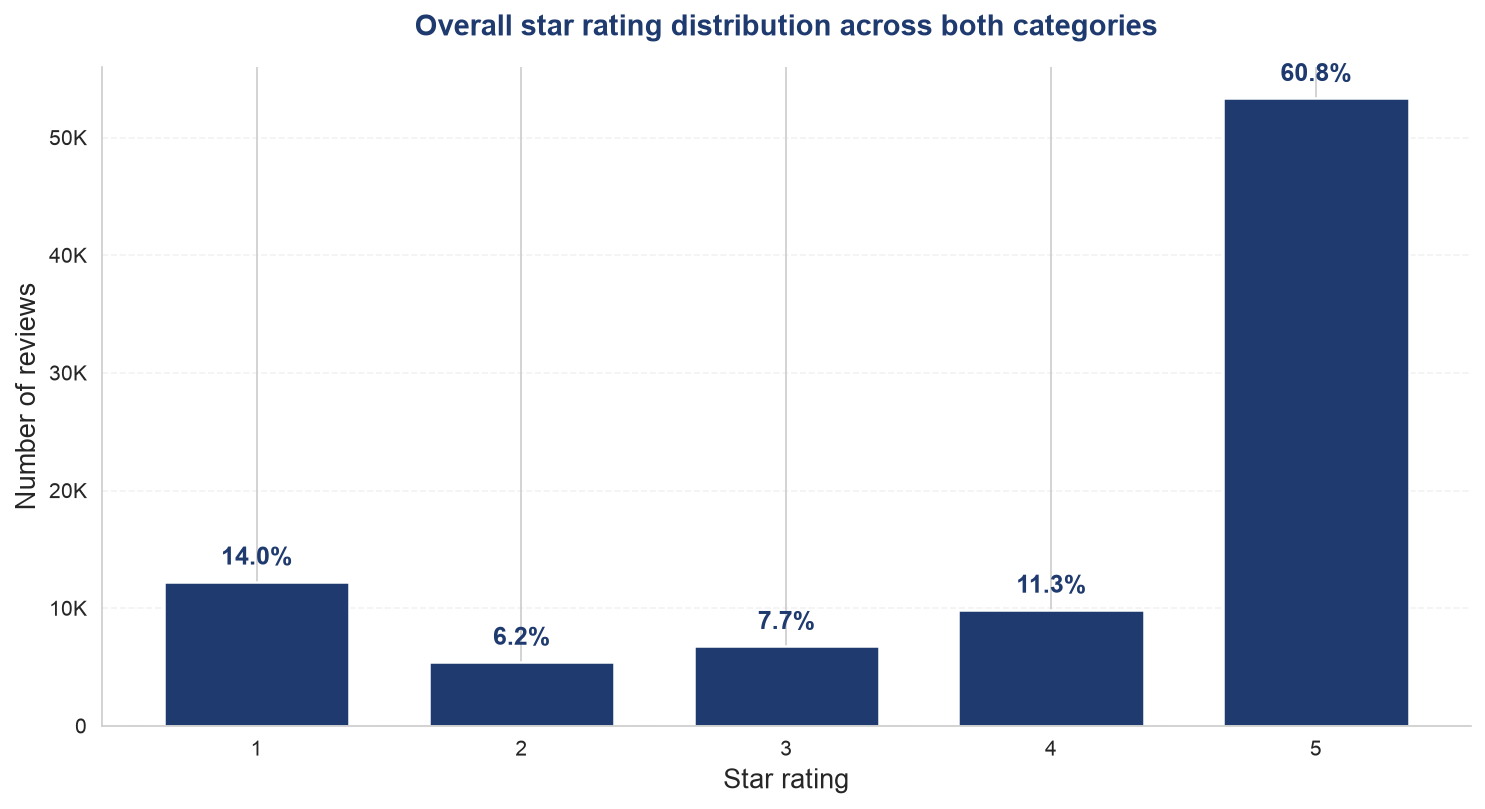
\includegraphics[width=\linewidth]{star_distribution_overall.png}
  \caption{Overall star distribution.}
\end{subfigure}\hfill
\begin{subfigure}{0.49\textwidth}
  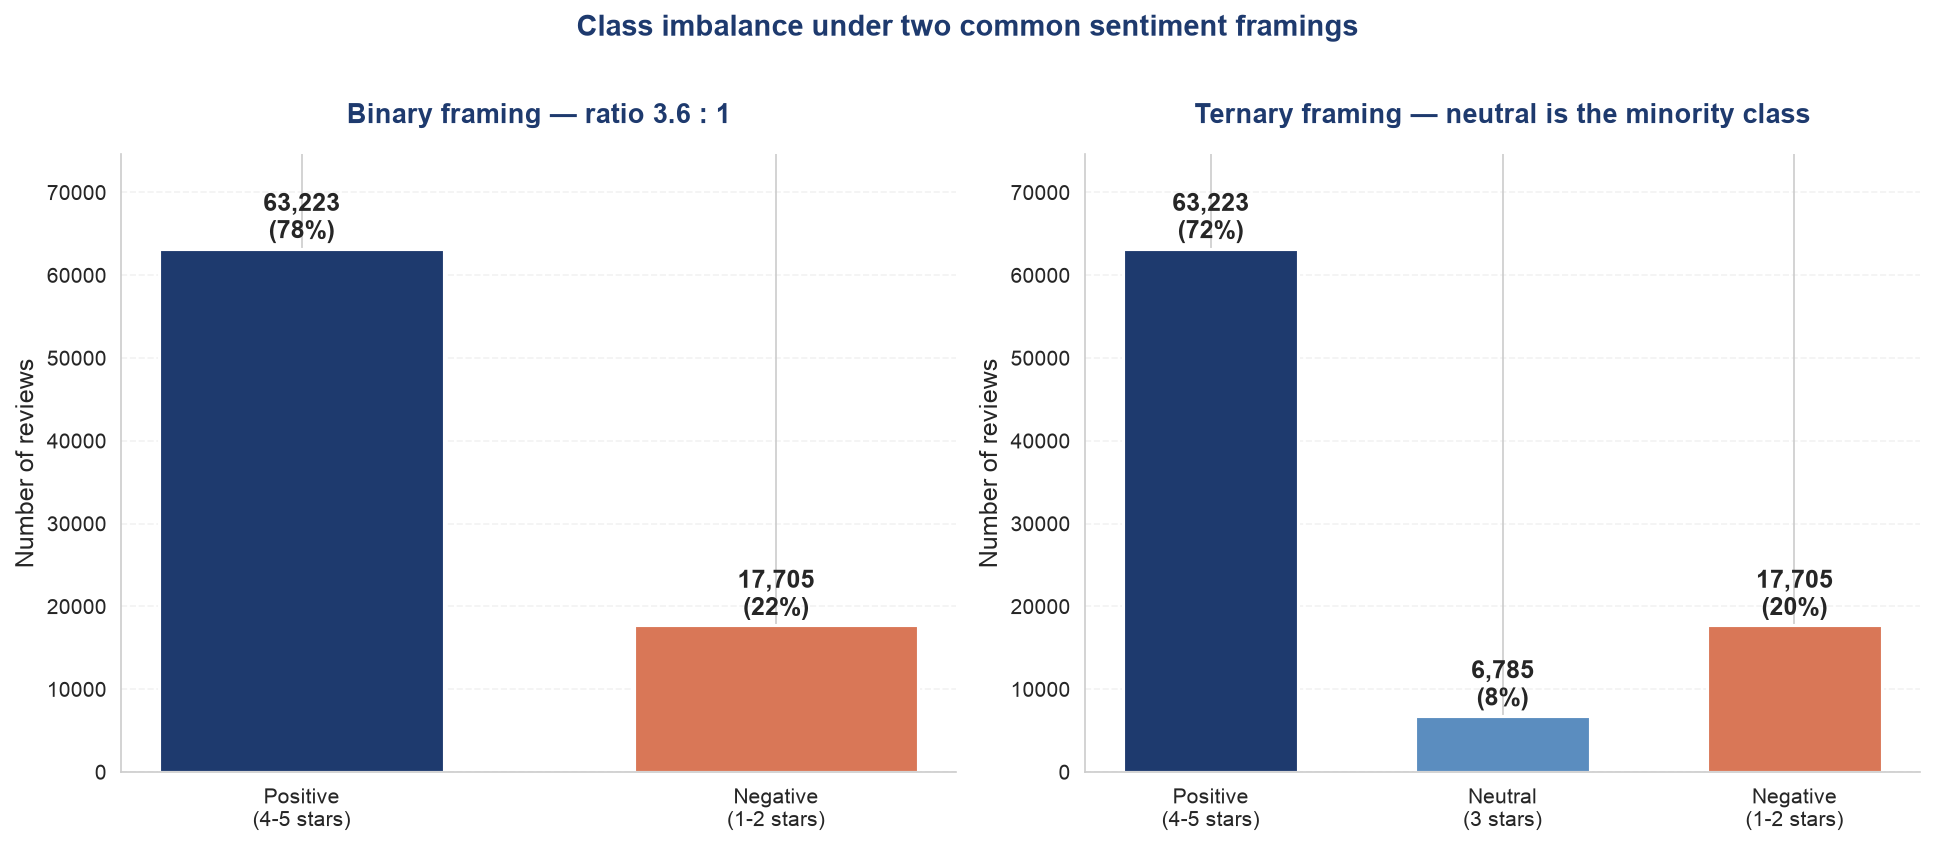
\includegraphics[width=\linewidth]{class_imbalance.png}
  \caption{Sentiment class imbalance.}
\end{subfigure}
\caption{Star ratings are heavily skewed toward 5 stars, producing a substantial
positive/negative imbalance and a small neutral class.}
\label{fig:stars}
\end{figure}

\begin{figure}[H]
\centering
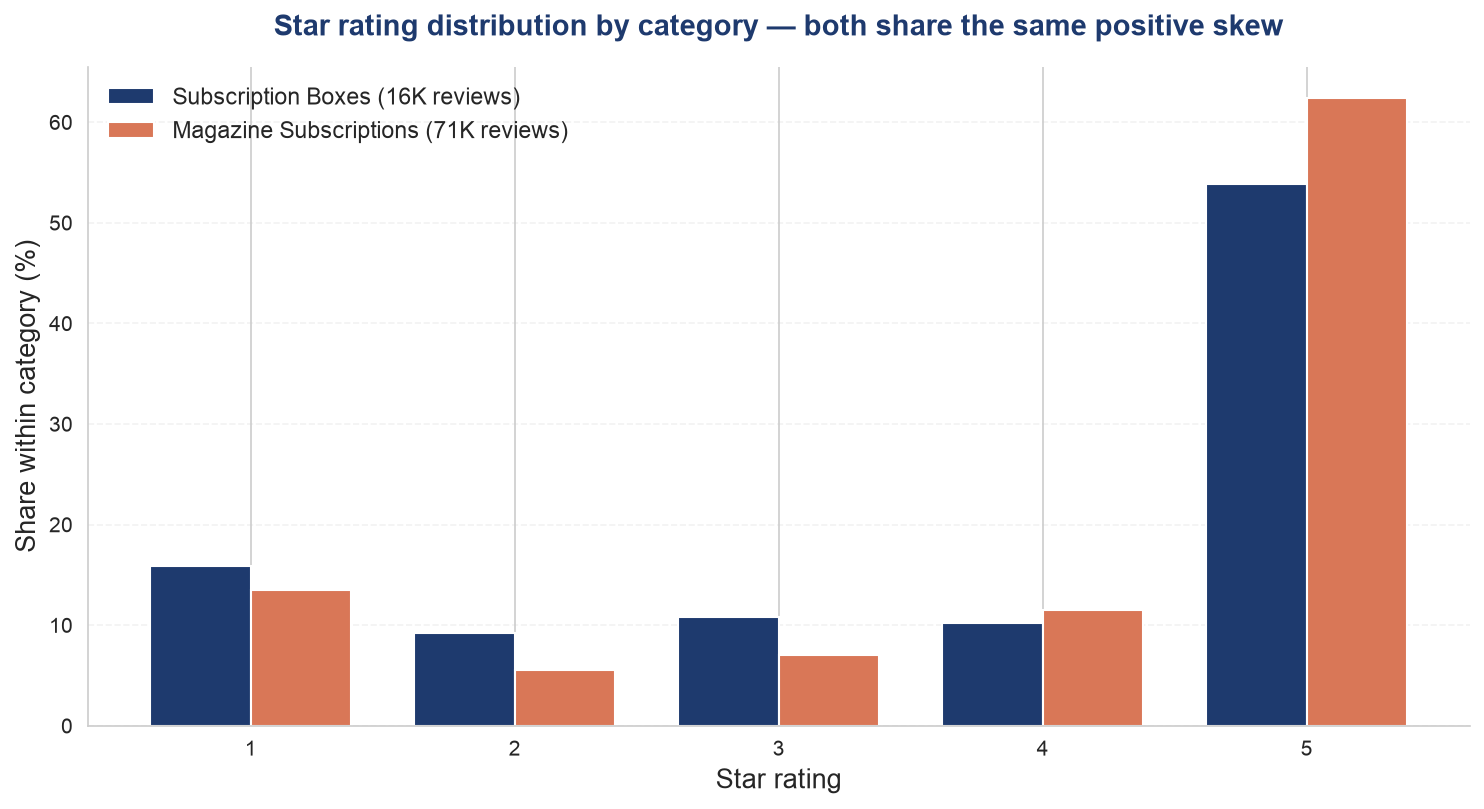
\includegraphics[width=0.62\textwidth]{star_distribution_by_category.png}
\caption{Per category star distribution: both categories share the positive
skew, confirming the imbalance is not an artefact of one category.}
\label{fig:imbalance}
\end{figure}

\subsection{Review length and vocabulary}
Reviews are short: a median of 22 words and a mean of 40 (Figure
\ref{fig:length}). Short texts carry few features, which both favours sparse
linear models and motivates the sentence level treatment in RQ2. A
whitespace tokenised vocabulary on a 20K review sample contains $6{,}308$ terms
with sample corpus frequency at least five. This is a descriptive corpus
statistic; the actual TF-IDF unigram feature count on the training split is
reported separately in Section \ref{sec:rq1}.

\begin{figure}[H]
\centering
\begin{subfigure}{0.49\textwidth}
  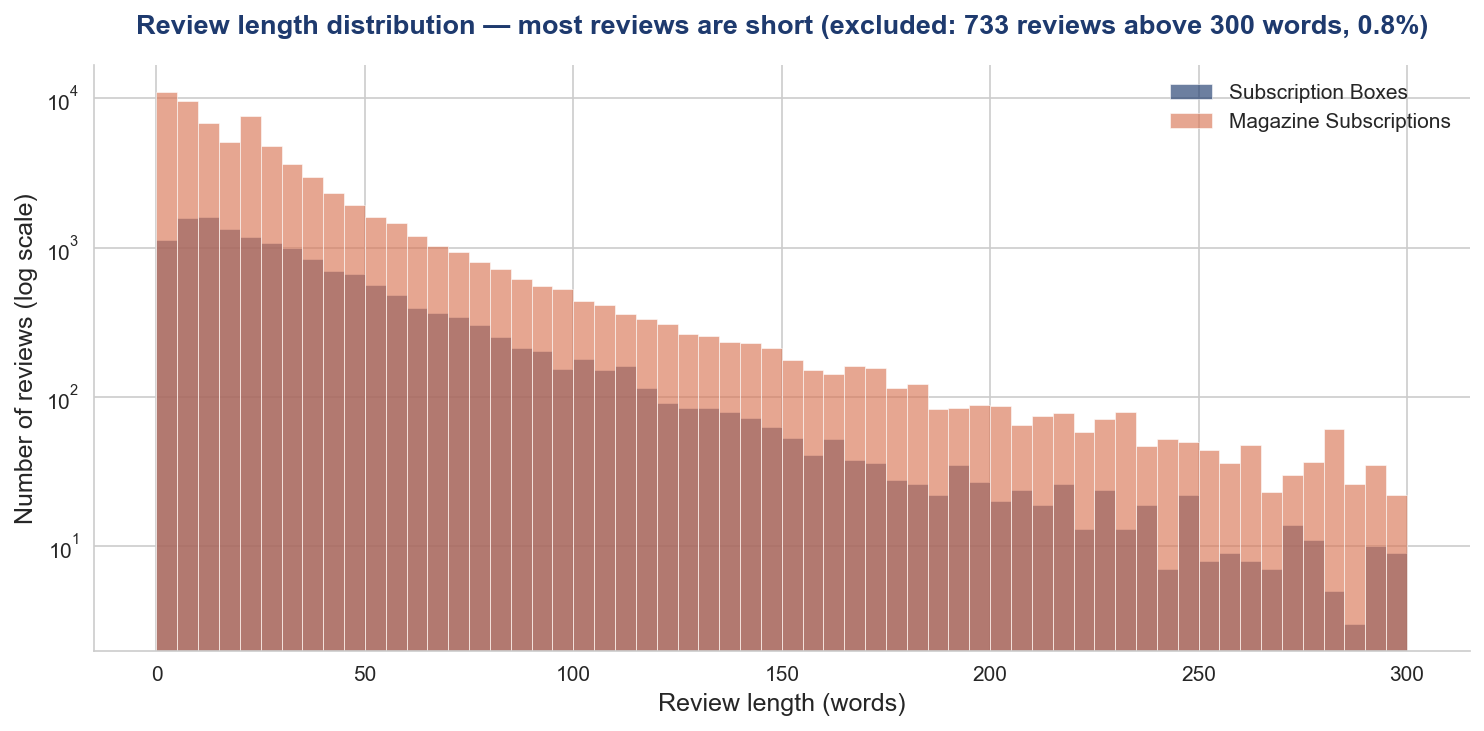
\includegraphics[width=\linewidth]{review_length_histogram.png}
  \caption{Review length distribution (words).}
\end{subfigure}\hfill
\begin{subfigure}{0.49\textwidth}
  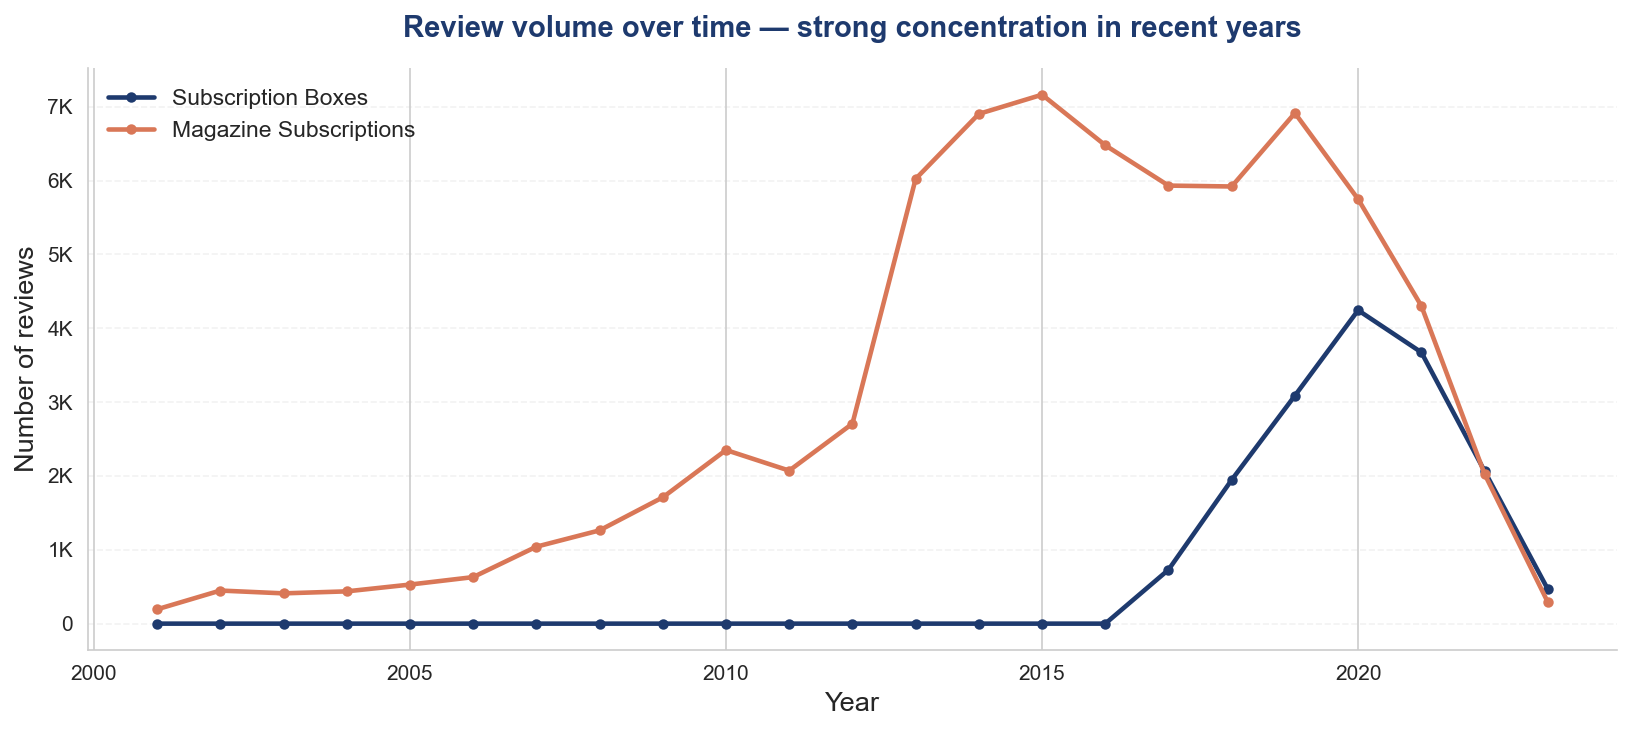
\includegraphics[width=\linewidth]{reviews_over_time.png}
  \caption{Review volume over time.}
\end{subfigure}
\caption{Most reviews are short, and review volume is concentrated in recent
years, which motivates a chronological rather than random train and test split.}
\label{fig:length}
\end{figure}

\subsection{Discriminative terms}
A weighted log odds analysis with an informative Dirichlet prior
\citep{monroe2008fightin} identifies the terms most associated with each
sentiment class. Rendered as word clouds (Figure \ref{fig:wordcloud}), the
positive class is dominated by generic affect (love, great, enjoy,
wonderful), while the negative class is strikingly concrete: cancel,
refund, subscription, ad, advertisement, charge, renewal. Already at the
descriptive stage, the data points to billing and advertising as the negative
themes that the modelling later confirms.

\begin{figure}[H]
\centering
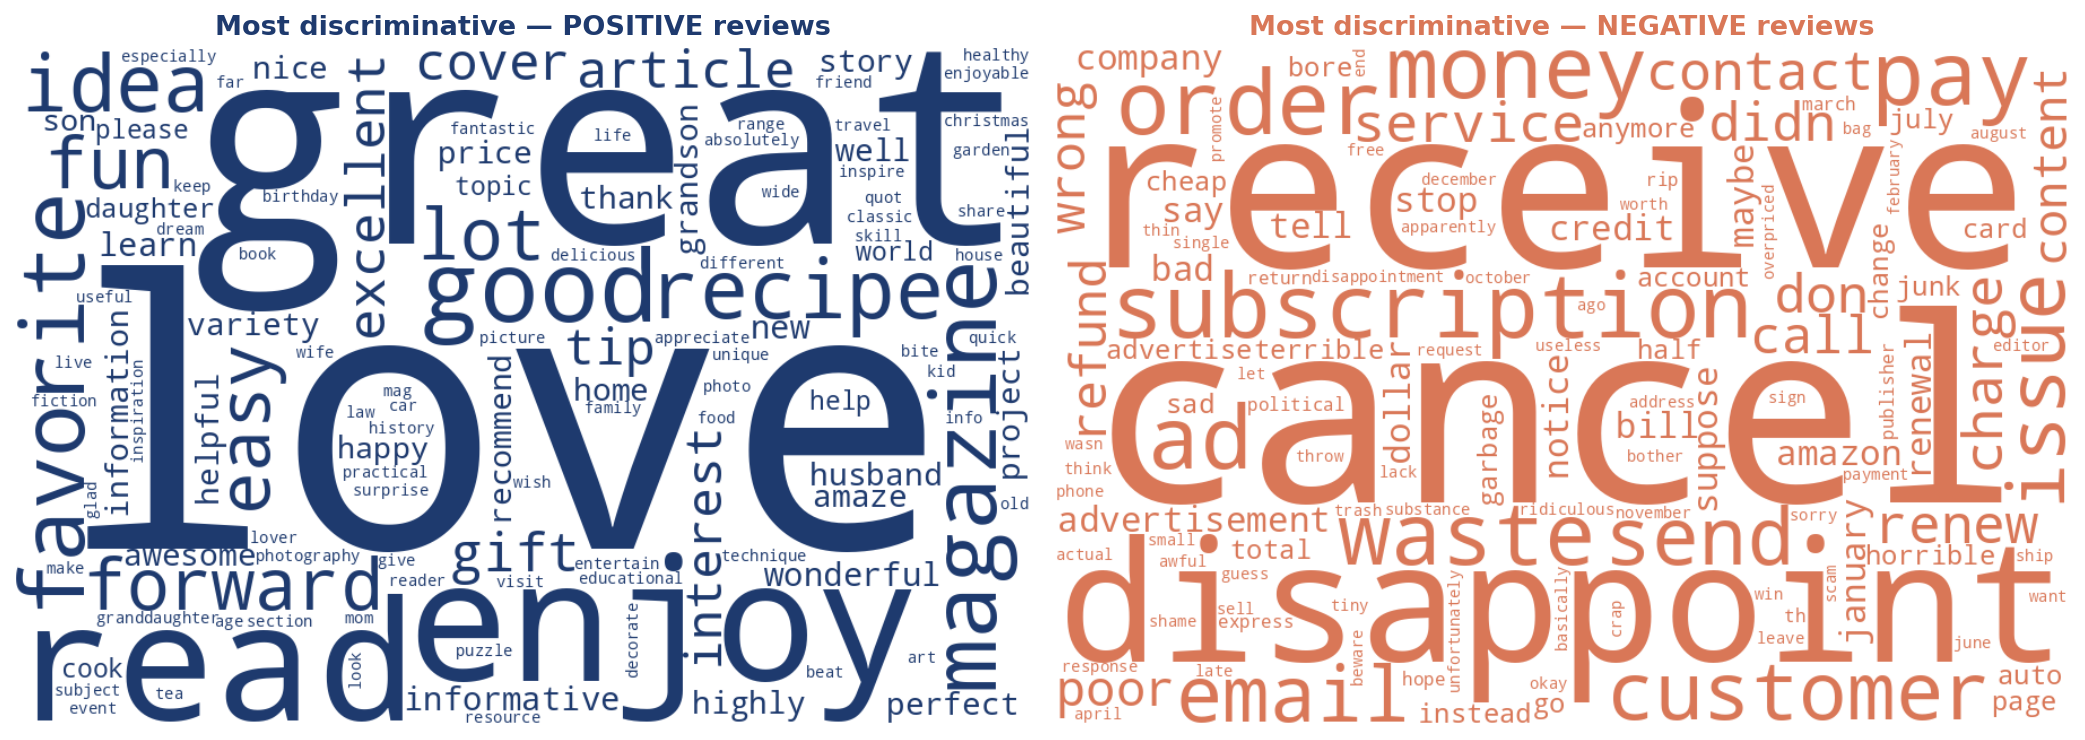
\includegraphics[width=\textwidth]{wordcloud_sentiment.png}
\caption{Most discriminative terms per sentiment class (size $\propto$ weighted
log odds z score). The negative cloud is a billing and advertising cluster.}
\label{fig:wordcloud}
\end{figure}

% ============================ 4 METHOD ======================================
\section{Methodology}
\label{sec:method}

\subsection{Sentiment labelling}
\label{sec:method-label}
Star ratings are the natural supervision signal but exist only per review, so
RQ1 operates at the document level. We use two framings. The binary
framing maps 1 to 2 stars to negative, 4 to 5 to positive and drops
3 star reviews; the ternary framing keeps 3 stars as neutral.
Binary leads the analysis; ternary is reported to probe the hard, mixed sentiment
middle.

\subsection{Text preprocessing}
The body text is lowercased and stripped of HTML, URLs and nonalphabetic
characters, then tokenised, stopword filtered and lemmatised with spaCy
(\texttt{en\_core\_web\_sm}). A small number of reviews ($238$) reduce to an
empty string and are dropped before modelling, as they carry no bag of words
signal. The cleaned text feeds only the TF-IDF classifiers of RQ1; VADER in RQ2
deliberately consumes the raw text, because its valence rules exploit
capitalisation, punctuation and intensifiers.

\subsection{Chronological split without test set leakage}
\label{sec:method-split}
Because review volume is concentrated in recent years, a random split would let a
model train on future reviews \citep{sculley2015hidden}. We therefore sort by
timestamp and split within each category so both categories appear on
every slice, preserving the cross category comparison RQ2 needs. Chronological
order is therefore preserved within each category; because the
per category splits are then combined into one development, validation and test set
for the joint classifier, the resulting combined train and test periods
partially overlap across categories (e.g.\ the combined training set can
contain Magazine Subscriptions reviews newer than some Subscription Boxes
reviews in the combined test set). The temporal guarantee this
split provides is therefore within category, not global: no review
trains a model on data from its own category's future, but the combined
classifier is not guaranteed to be evaluated on a period strictly later than
all of its combined training data across categories.

A plain oldest 80\% and newest 20\% split is not enough on its own: if the held out
20\% is inspected repeatedly while comparing features, imbalance handling and
hyperparameters, the final reported number is no longer an honest estimate of
out of sample performance. We therefore split further into oldest
64\% (development training), next 16\% (validation), and newest
20\% (final test). Feature representation (unigram vs.\ uni+bigram),
imbalance handling, and a small deterministic hyperparameter grid: Naive
Bayes $\alpha\in\{0.1,0.5,1.0,2.0\}$ crossed with \{no handling, reproducible
undersampling\}; Logistic Regression $C\in\{0.1,0.5,1.0,2.0,5.0\}\times
\text{class\_weight}\in\{\text{none},\text{balanced}\}$; Gradient Boosting
$n_{\text{estimators}}\in\{40,80\}\times\text{learning\_rate}\in\{0.05,0.1\}
\times\text{max\_depth}\in\{2,3\}\times\text{class\_weight}\in\{\text{none},
\text{balanced}\}$ are all selected using only the validation slice,
by validation macro-F1 (primary) with minority class recall as a transparent
tie breaker. The selected configuration is then retrained on the full oldest
80\% (development training plus validation) and evaluated on the final 20\%. Final test
labels, predictions and performance metrics are never used for model,
feature or hyperparameter selection; they are computed exactly once, after
every modelling choice above has been fixed. This is distinct from the
descriptive exploratory analysis (Section \ref{sec:eda}), which inspects the
full dataset including the test period and so, unlike the modelling
decisions above, was not shielded from the test period. This is acceptable for
descriptive EDA, but worth keeping separate from the leakage free claim about
model selection.

\subsection{Features}
We build TF-IDF vectors with sublinear term frequency scaling, $\mathrm{min\_df}=5$
and a vocabulary cap of $20{,}000$. Two configurations are compared: unigrams,
and unigrams+bigrams; the vectoriser is fit on the training split only, and the
choice between them is made on the validation slice (Section
\ref{sec:method-split}), not on the final test set.

\subsection{Models and imbalance handling}
We evaluate a majority class baseline (always predicts positive),
Multinomial Naive Bayes, Logistic Regression and
\texttt{sklearn.ensemble.GradientBoostingClassifier}
\citep{friedman2001greedy,pedregosa2011scikit}. Imbalance is handled two ways:
Logistic Regression uses \texttt{class\_weight=balanced}; Gradient Boosting uses
balanced sample weights in the fitted sample; Naive Bayes, which has no
class weight parameter, is trained on a randomly undersampled balanced set
rather than SMOTE \citep{chawla2002smote}, which we consider methodologically
debatable in a sparse, high dimensional TF-IDF space (Section
\ref{sec:related-imbalance}). Each model is also run without handling so the
effect of imbalance is directly visible. The selected Gradient Boosting
configuration is trained on a deterministic stratified sample of $12{,}000$
reviews regardless of how much training data is available, for tractable
reproduction; this cap, and its consequence for the fairness of any
full data comparison, is reported transparently (Section \ref{sec:rq1-fair}).

\subsection{Fair model family comparison}
\label{sec:method-fair}
Because Gradient Boosting trains on at most 12,000 rows while Naive Bayes and
Logistic Regression can use the full training pool, a naive full data
comparison would conflate model family capability with
training data volume. We therefore report two distinct blocks on the
final test set: a matched sample comparison, in which all three
families train on an identical, deterministically sampled 12,000 row training
set, and a full data comparison (Naive Bayes and Logistic Regression
only; Gradient Boosting is excluded because its 12,000 row cap means a
``full data'' run would not actually reflect more training data than the
matched comparison).
The matched sample block equalises the final training rows; hyperparameter
selection, however, was conducted under each model's operational training
regime (full development training for Naive Bayes and Logistic Regression, the internal
12,000 row cap for Gradient Boosting). We do not quantify the effect of this
asymmetry, so it is not used to support any claim about general model family
superiority.

\subsection{Evaluation and uncertainty}
We report accuracy (for reference), macro averaged F1, weighted F1 and per class
recall, plus confusion matrices. Macro-F1 and minority class recall are the
primary metrics under imbalance. All final test metrics are additionally
reported with nonparametric bootstrap 95\% confidence intervals (2,000
replications, fixed seed, percentile method) following \citet{efron1993bootstrap},
stratified by true class for per class recall. The unigram versus bigram comparison
uses a paired bootstrap (same resampled indices for both feature
configurations in every replication) so the reported difference and its CI are
directly comparable; if the CI excludes zero we describe a stable difference
under this holdout, and if it includes zero we describe only a small observed
gain, not a confirmed or significant improvement. Error analysis ranks the most
confidently wrong predictions to characterise the hardest reviews, using a
rule based exploratory categorisation rather than manual coding.

\subsection{Aspect based pipeline (RQ2)}
\label{sec:method-rq2}
A review level label cannot express that one review praises content but
criticises price, so RQ2 works below the review. Each review is split into
sentences; aspects are detected per sentence using a curated keyword lexicon of
eight aspects: delivery, packaging, quality, price, content, customer
service, billing and advertising. The last three are domain specific:
EDA surfaced content, billing/renewal and advertising vocabulary prominently.
To avoid circularity, the detection lexicon contains aspect nouns/actions rather
than sentiment words, and it excludes broad product identifiers such as
box, magazine and subscription. A complementary, lexicon free
noun phrase view (spaCy noun chunks) provides data driven aspect candidates.
Each aspect mentioning sentence is scored with VADER \citep{hutto2014vader}, and
scores are aggregated per review, per aspect and per category.

\paragraph{Why VADER rather than the RQ1 classifier.}
The RQ1 classifier is trained on whole reviews; applying it to single sentences
is an out of distribution use, since sentences are far shorter with a different
feature distribution. VADER needs no training and is built for short text, so it
is the primary sentence level scorer. The document classifier is retained
only as a robustness check: we measure how often the two methods agree
rather than assuming either is ground truth (Section \ref{sec:rq2-robust}).

\paragraph{Defining ``high coverage'' / ``substantial''.}
\label{sec:method-coverage}
Prior drafts called aspects ``substantial'' or ``high coverage'' without a
fixed rule. We define an aspect as high coverage within a category if and only if
at least 5\% of that category's reviews mention it, and apply this single
threshold consistently in the methodology, results, discussion and conclusion.

\paragraph{Clause level sensitivity analysis.}
Sentence level attribution cannot separate two aspects that cooccur in one
sentence with mixed sentiment (``great content \dots but overpriced''): both
inherit the sentence's single VADER score. As a sensitivity check on this
limitation, not a replacement for the sentence level primary method, we
additionally split sentences conservatively into clauses on a semicolon or one
of but, however, although, though, yet, while, whereas, and attribute
each aspect only to the clause(s) that contain its keyword (Section
\ref{sec:rq2-clause}).

\paragraph{Billing lexicon sensitivity check.}
The billing keyword list contains words such as cancel, refund
and charged that often already occur in problem oriented contexts. We
check (a)~each billing keyword's own VADER valence in isolation, and (b)~billing
sentiment recomputed with the matched keyword masked out before scoring,
compared against the unmasked score (Section \ref{sec:rq2-lexicon-check}). This
is a leakage and lexicon sensitivity check, not an alternative primary method.

\paragraph{Review level bootstrap uncertainty.}
The aspect sentence table has multiple rows per review (one per mentioned
aspect, occasionally more), so rows are not independent observations. We
therefore resample whole reviews, not individual rows, for bootstrap 95\%
CIs of mean aspect sentiment per category and of the cross category difference
(2,000 replications, fixed seed; Section \ref{sec:rq2-uncertainty}).

% ============================ 5 RESULTS RQ1 =================================
\section{Results: Document Level Sentiment (RQ1)}
\label{sec:rq1}

All model, feature and hyperparameter decisions in this section were made on
a held out validation slice (16\% of the data) and never on the
final test set; after those decisions were fixed, the selected configuration,
Logistic Regression, \texttt{class\_weight=balanced}, uni+bigram features,
was retrained on the full oldest 80\% and evaluated on the final 20\% test set
(Section \ref{sec:method-split}). The validation only grid search confirmed
this same configuration as the best performer in both framings, ahead of every
Naive Bayes and Gradient Boosting configuration tried, before the final
test set was inspected.

\subsection{Binary and ternary framings}
Table \ref{tab:rq1demo} (full 14 row grid in Appendix \ref{app:val})
illustrates why imbalance handling matters,
using the validation slice (not the final test set, and not used for any
selection decision). In both framings the majority baseline has zero
recall on the class(es) it never predicts; without handling, Naive Bayes'
neutral recall collapses to $0.8\%$ in the ternary framing, and Logistic
Regression's negative/neutral recall stays low ($0.69$/$0.12$). Balancing or
undersampling lifts minority recall substantially in both framings, at a real
accuracy cost in the ternary case.

\begin{table}[H]
\centering
\caption{RQ1 imbalance handling demonstration, best and worst case per framing
(validation slice, illustrative only; full 14 row grid in Appendix
\ref{app:val}).}
\label{tab:rq1demo}
\setlength{\tabcolsep}{4pt}
\begin{tabular}{llrrrrr}
\toprule
Framing & Model & Acc. & Macro-F1 & Rec$_{\text{pos}}$ & Rec$_{\text{neu}}$ & Rec$_{\text{neg}}$ \\
\midrule
Binary & Majority baseline           & 0.776 & 0.437 & 1.000 & --    & 0.000 \\
Binary & Log.\ Reg.\ (balanced) & 0.918 & 0.888 & 0.926 & -- & 0.889 \\
\midrule
Ternary & Majority baseline          & 0.719 & 0.279 & 1.000 & 0.000 & 0.000 \\
Ternary & Log.\ Reg.\ (balanced) & 0.813 & 0.651 & 0.880 & 0.449 & 0.712 \\
\bottomrule
\end{tabular}
\end{table}

On the final test set, accessed only after selection, the chosen binary
configuration reaches accuracy $0.902$, macro-F1 $0.888$,
recall$_{\text{pos}}=0.910$, recall$_{\text{neg}}=0.884$; by category,
macro-F1 is $0.894$ for Magazine Subscriptions and $0.858$ for Subscription
Boxes (negative recall $0.881$/$0.903$). The combined classifier is not
simply learning the larger category at the expense of the smaller one. The
selected ternary configuration ($C{=}0.5$, balanced) reaches accuracy
$0.785$, macro-F1 $0.644$, recall$_{\text{pos}}=0.848$,
recall$_{\text{neu}}=0.448$, recall$_{\text{neg}}=0.731$ (95\% bootstrap CIs
for both framings in Table \ref{tab:rq1bootstrap}; confusion matrices in
Figure \ref{fig:rq1conf}). This is the central RQ1 trade off: the 3 star class
shows persistent difficulty under the evaluated setup on every
held out slice we tried (not a provable, universal ceiling) because such
reviews genuinely mix positive and negative content. This directly motivates
both the dedicated 3 star analysis below (Section \ref{sec:rq1-3star}) and the
sentence level view of RQ2.

\begin{figure}[H]
\centering
\begin{subfigure}{0.58\textwidth}
  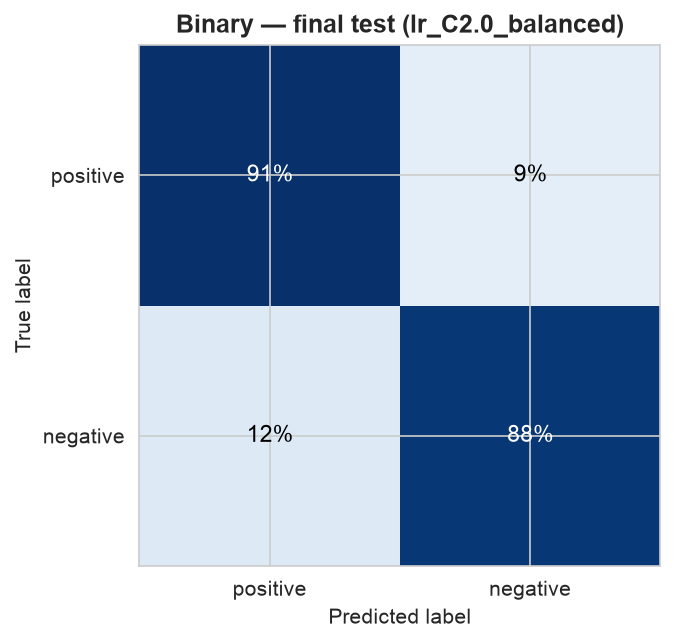
\includegraphics[width=\linewidth]{rq1_confusion_binary.png}
  \caption{Binary.}
\end{subfigure}\hfill
\begin{subfigure}{0.4\textwidth}
  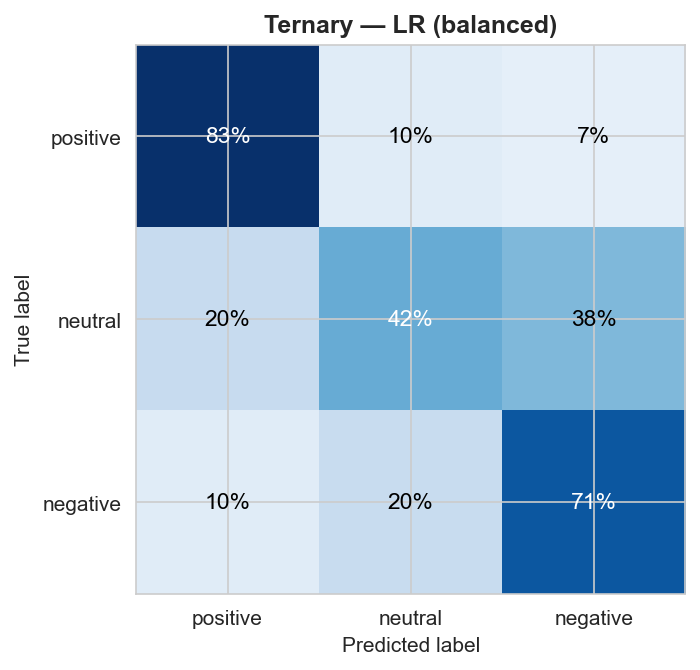
\includegraphics[width=\linewidth]{rq1_confusion_ternary.png}
  \caption{Ternary.}
\end{subfigure}
\caption{Final test set confusion matrices, selected configuration. Neutral
reviews (ternary) are most often confused with the adjacent positive class.}
\label{fig:rq1conf}
\end{figure}

\subsection{Statistical uncertainty}
\label{sec:rq1-uncertainty}
Table \ref{tab:rq1bootstrap} reports 95\% class stratified bootstrap
confidence intervals (2,000 replications, fixed seed) for every final test
metric above: each replication resamples within each true class stratum at
that stratum's original size (Section \ref{sec:method-split}), so class
proportions are fixed across replications rather than also varying by chance.
For the unigram versus bigram comparison, both configurations were retrained on
the full oldest 80\% and evaluated on the final test set with a
paired, equally stratified bootstrap (same resampled indices for
both): macro-F1 is $0.875$ (unigram) vs.\ $0.888$ (uni+bigram), difference
$+0.013$, 95\% CI $[0.009, 0.016]$. Because this CI excludes zero, we describe
this as a stable, if modest, difference under this holdout, not a
``real'' or independently significance tested improvement, since no formal
hypothesis test was run beyond the percentile bootstrap CI itself. The core
CIs are: binary accuracy $0.902$ $[0.897, 0.906]$, binary macro-F1 $0.888$
$[0.883, 0.893]$; ternary macro-F1 $0.644$ $[0.636, 0.652]$, ternary
recall$_{\text{neu}}$ $0.448$ $[0.421, 0.475]$. The full 9 row table (all
metrics, both framings) is in Appendix \ref{app:val}, Table \ref{tab:rq1bootstrap}.

\subsection{Fair model family comparison}
\label{sec:rq1-fair}
Because the selected Gradient Boosting configuration trains on at most
12,000 rows, a full data comparison against Naive Bayes and Logistic
Regression (trained on $64{,}456$ rows) would conflate model family capability
with training data volume. Table \ref{tab:rq1fair} reports two blocks on the
final test set: a matched sample comparison (all three families on an
identical, deterministically sampled 12,000 row training set) and a
full data comparison (Naive Bayes and Logistic Regression only;
Gradient Boosting is omitted because its internal 12,000 row cap means a
``full data'' run would not reflect more training data than the matched
comparison and would misrepresent the result as a scaling finding).

\begin{table}[H]
\centering
\caption{Fair model family comparison, binary framing, final test set. Each
model uses its own validation selected hyperparameters (Section
\ref{sec:method-split}); Naive Bayes' $n_{\text{train}}$ in Block B is below
$64{,}456$ because its validation selected configuration uses undersampling.}
\label{tab:rq1fair}
\begin{tabular}{llrrrr}
\toprule
Block & Model & $n_{\text{train}}$ & Accuracy & Macro-F1 & Recall$_{\text{neg}}$ \\
\midrule
Matched (A) & Naive Bayes           & 12{,}000 & 0.855 & 0.814 & 0.616 \\
Matched (A) & Logistic Regression   & 12{,}000 & 0.891 & 0.876 & 0.858 \\
Matched (A) & \texttt{GradientBoostingClassifier} & 12{,}000 & 0.841 & 0.815 & 0.750 \\
\midrule
Full data (B) & Naive Bayes         & 25{,}230 & 0.870 & 0.857 & 0.909 \\
Full data (B) & Logistic Regression & 64{,}456 & 0.902 & 0.888 & 0.884 \\
\bottomrule
\end{tabular}
\end{table}

Logistic Regression wins even in the matched sample block, where
every model family trains on identical data, so its advantage is not an
artefact of Gradient Boosting receiving less training data, though the margin
over Naive Bayes is narrower than a naive (non validation tuned) Naive Bayes
baseline would suggest once Naive Bayes is also given its own
validation selected hyperparameters. Combined with
Block B, this supports calling Logistic Regression the strongest
observed model under the evaluated setup, but the unequal full data training
sizes between Logistic Regression and Gradient Boosting are never, by
themselves, used as evidence that linear models are categorically superior to
gradient boosting in general.

\subsection{Feature representation}
The choice between unigrams and uni+bigrams was made on the validation slice
(Table \ref{tab:feat}): bigrams roughly double the vocabulary for a small
observed macro-F1 gain in both framings. The final test paired bootstrap
verdict for this gain is reported in Section \ref{sec:rq1-uncertainty} above.
A vocabulary sanity check confirms that $1{,}338$ negation bearing unigram/bigram
features (e.g.\ not worth, absolutely not) survive preprocessing
and enter the final TF-IDF vocabulary.

\begin{table}[H]
\centering
\caption{Feature comparison on the validation slice (Logistic Regression,
balanced).}
\label{tab:feat}
\setlength{\tabcolsep}{4.5pt}
\begin{tabular}{lrrrr}
\toprule
& \multicolumn{2}{c}{Binary} & \multicolumn{2}{c}{Ternary} \\
\cmidrule(lr){2-3}\cmidrule(lr){4-5}
Features & \#\,Feat. & Macro-F1 & \#\,Feat. & Macro-F1 \\
\midrule
TF-IDF unigram        & 8{,}341  & 0.872 & 8{,}819  & 0.636 \\
TF-IDF uni+bigram     & 20{,}000 & 0.888 & 20{,}000 & 0.651 \\
\bottomrule
\end{tabular}
\end{table}

\subsection{Interpretability}
A linear TF-IDF model exposes a signed weight per feature. Figure
\ref{fig:coef} visualises the strongest weights from the final selected binary
model, with the exact coefficient table in Appendix Table \ref{tab:coef}. The
positive weights are generic affect; the negative weights are dominated by negation cues and domain specific
terms such as disappointed, cancel, disappointing, poor and the
bigram cancel subscription. The strongest overall negative coefficient is
not, which confirms that preserving negation matters. Among the
domain specific terms, cancel is the strongest billing signal and the
fifth largest negative coefficient overall, a feature level precursor to the
RQ2 billing result, read as complementary rather than independently
confirmatory evidence (Section \ref{sec:discussion}).

\begin{figure}[H]
\centering
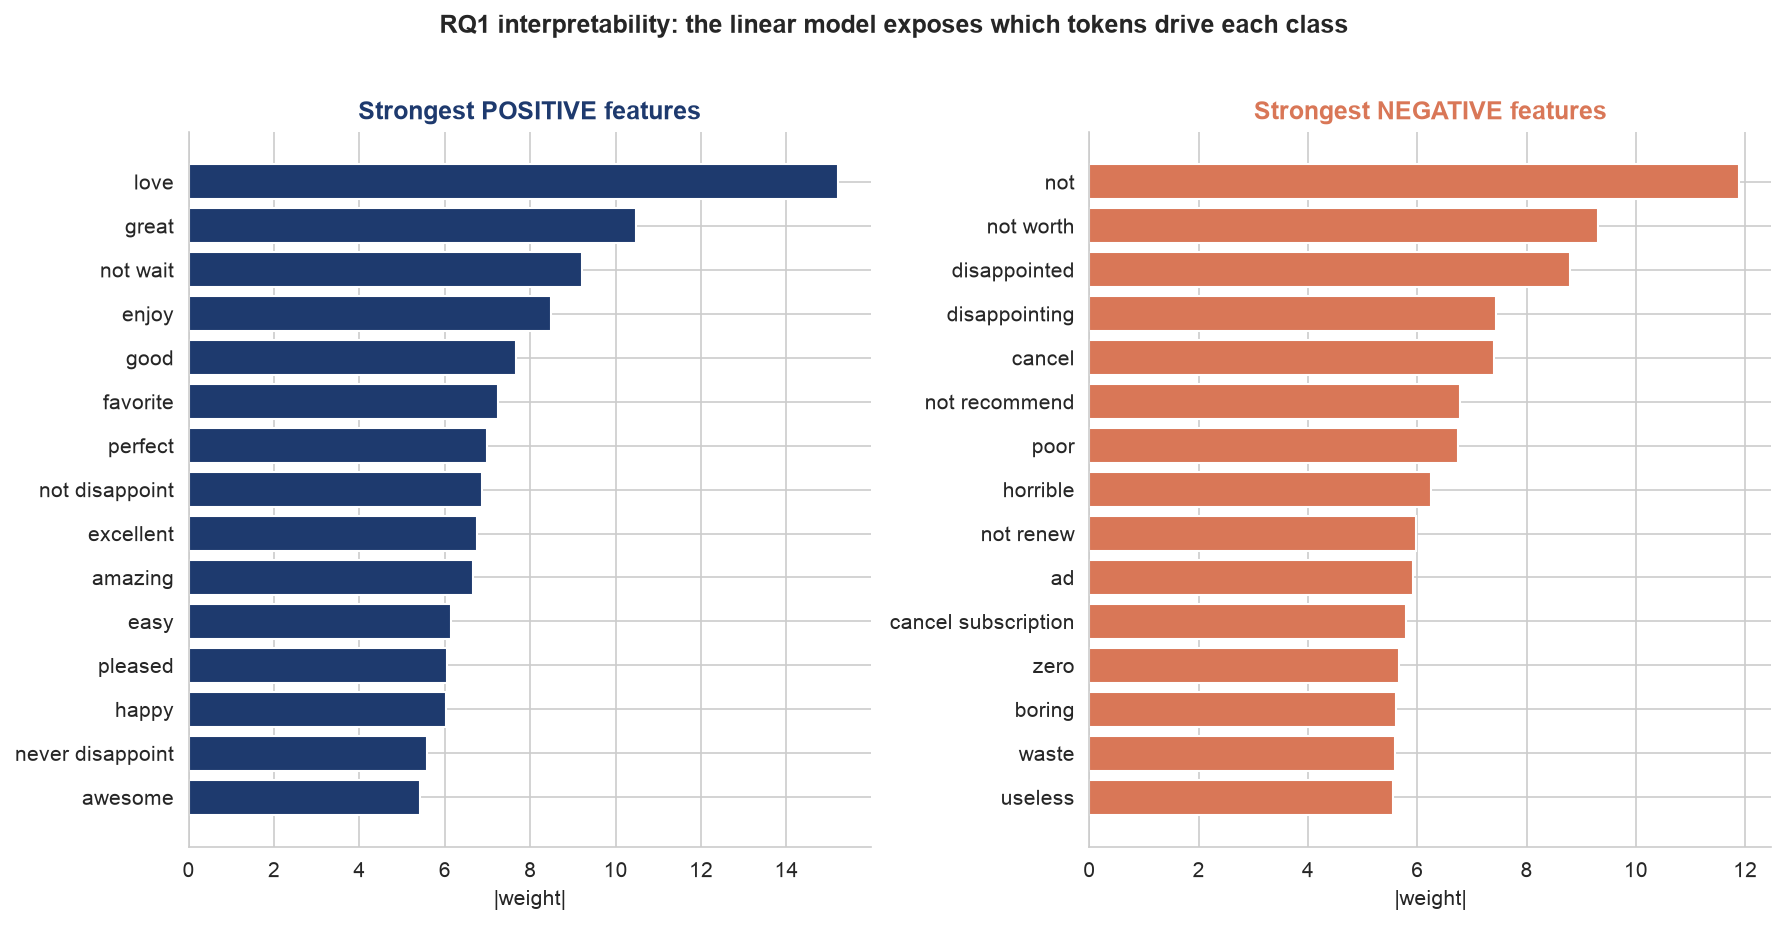
\includegraphics[width=\textwidth]{rq1_lr_coefficients.png}
\caption{The linear model is fully auditable: each token carries an explicit,
signed contribution to the positive/negative decision.}
\label{fig:coef}
\end{figure}

\subsection{Error analysis: the hardest reviews}
Ranking the most confidently wrong Logistic Regression predictions (final test
set) reveals that several errors appear to reflect disagreement between the
rating and the review text rather than a simple preprocessing failure. To make
this less anecdotal, the 100 highest confidence binary errors were grouped with
a rule based exploratory categorisation (Appendix Table
\ref{tab:err}), using simple keyword and length heuristics written by the author, not a
validated manual taxonomy and not human coded data. The category named
``potential rating text disagreement / possible label noise candidate''
deliberately avoids asserting that these cases are confirmed label noise. The
heuristic suggests that such disagreement candidates form the largest group
($47$ of $100$), followed by very short or context free reviews ($25$) and mixed
sentiment ($14$), but it is not a precise population estimate of how often label
noise occurs in the dataset.

\subsection{Direct analysis of 3 star reviews}
\label{sec:rq1-3star}
The binary error analysis above never includes 3 star reviews (dropped under
that framing). This section directly analyses all $1{,}248$ reviews with true
rating 3 in the final test set, using the selected ternary model. This is a
reproducible, automatic exploratory analysis (contrastive marker and
lexical cue word lists), not manual coding, and introduces no manual labels.

The model predicts neutral for $44.8\%$ of true 3 star reviews (matching the
ternary neutral recall above), negative for $38.5\%$, and positive for only
$16.7\%$. The model's confusion skews toward negative, consistent with
3 star reviews often reading as mild complaints (Figure \ref{fig:rq1threestar}).
Mean predicted class confidence is similar across all three predicted classes
($0.61$ to $0.63$) and barely differs between correct and incorrect predictions,
so predicted probability alone is not a reliable signal for catching the
model's mistakes here. Incorrect predictions are on average modestly longer
than correct ones ($43.2$ vs.\ $40.6$ words). A contrastive marker
(but/however/although/though/yet/while/whereas) appears in $41.6\%$ of
3 star reviews regardless of correctness, so contrastive markers alone do not
strongly separate hard cases from easy ones in this automatic check; $18.4\%$
of 3 star reviews contain both a positive and a negative lexical cue from fixed
word lists, a direct automatic signature of mixed sentiment. Deterministically
selected representative examples (the two highest confidence 3 star reviews
predicted into each class, not manually curated) make the pattern concrete:
short enthusiastic 3 star reviews (``Love this!!!'') get predicted positive;
moderately worded genuine complaints (``The wording on this item was not
clear at purchase\dots{} Chatted to cancel and surprisingly got a partial
refund'') get predicted negative; and explicitly lukewarm/mixed language
(``Articles are somewhat interesting\dots{} Too many added advertisements'')
gets predicted neutral correctly. This directly answers the RQ1 subquestion on
mixed sentiment 3 star reviews: the limitation is not that the model is
unconfident on these reviews, but that bag of words features cannot reliably
separate mildly positive from mildly negative phrasing, and the star rating
itself is sometimes only loosely tied to the text.

\begin{figure}[H]
\centering
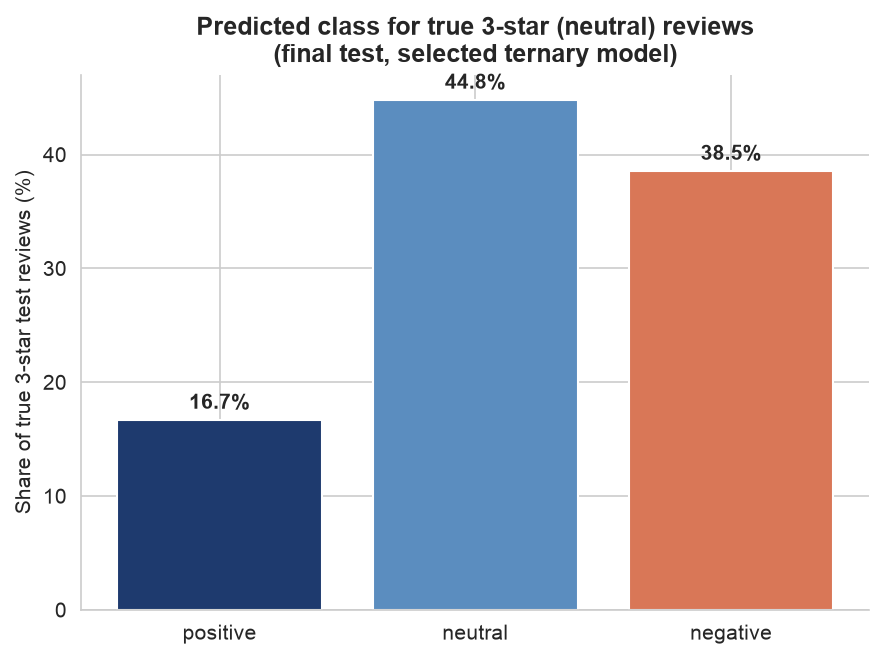
\includegraphics[width=0.55\textwidth]{rq1_3star_predicted_distribution.png}
\caption{Predicted class for true 3 star (neutral) reviews, final test set,
selected ternary model.}
\label{fig:rq1threestar}
\end{figure}

% ============================ 6 RESULTS RQ2 =================================
\section{Results: Aspect Based Sentiment (RQ2)}
\label{sec:rq2}

\subsection{What customers discuss}
Aspect mention rates differ sharply by category (Figure \ref{fig:rq2mention},
Table \ref{tab:rq2}). After cleaning the lexicon, content is the largest
aspect in both categories: $43.0\%$ of Subscription Box reviews and $38.5\%$ of
Magazine reviews mention product or editorial substance. Price and
delivery are secondary themes for boxes, while magazines show more
price and advertising discussion. Crucially, packaging now
appears in only $6.1\%$ of box reviews; the earlier high value was a product name
artefact caused by matching box/boxes, not evidence that packaging
dominates the category. Because Subscription Box reviews are on average longer
than Magazine reviews (Section \ref{sec:eda}), we also checked mentions per
100 words as a length normalised sensitivity view; the ranking of aspects by
discussion volume is materially unchanged (content remains the largest theme
in both categories), so the per review mention rate is retained as the
headline statistic.

\begin{figure}[H]
\centering
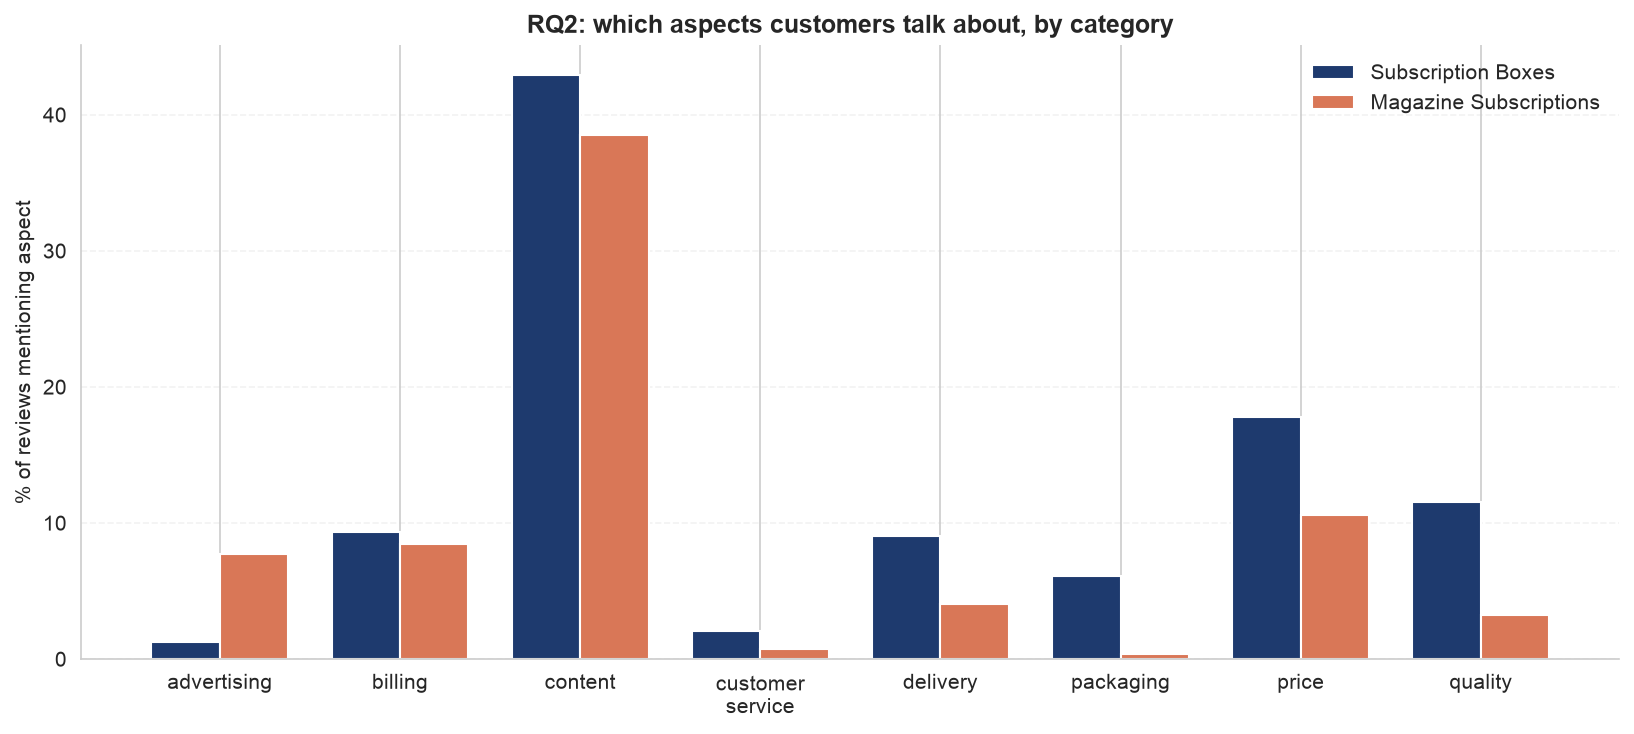
\includegraphics[width=0.9\textwidth]{rq2_mention_rate.png}
\caption{Share of reviews mentioning each aspect, by category. The cleaned
lexicon shows content as the largest aspect and removes the earlier packaging
artefact caused by product name matches.}
\label{fig:rq2mention}
\end{figure}

\subsection{Aspect sentiment}
The radar and bar views (Figures \ref{fig:rq2radar}, \ref{fig:rq2sent}) and
Table \ref{tab:rq2} agree on one pattern: billing is high coverage
(mention rate $\geq 5\%$, Section \ref{sec:method-coverage}) in both
categories and is the weakest high coverage aspect in both (compound
$-0.091$ for boxes, $0.051$ for magazines). For Subscription Boxes the raw
lexicon score is the lowest ($56.9\%$ negative share), but the masking check
below shows this polarity is not robust after removing trigger terms. For
Magazine Subscriptions the mean is only slightly above neutral, so we do
not describe billing there as an unconditionally negative pain point,
only as the weakest aspect among the high coverage ones. This is much sharper than the
earlier broad subscription version of the lexicon: once neutral product
mentions are removed, billing's negative skew for boxes becomes visible rather
than being diluted by neutral mentions. Content and quality are
the most positive high coverage aspects in boxes (compound $\approx
0.33$ to $0.34$), while magazines are most positive about content and
price (compound $\approx 0.32$ to $0.33$). Advertising is high coverage
only in magazines ($7.7\%$ mention rate) and is not the dominant pain point
there. The sentiment composition per aspect (Figure \ref{fig:rq2sent}) shows
the same pattern: billing carries the largest red (negative) band among
high coverage aspects. Customer service is numerically more negative in
Magazine Subscriptions ($-0.029$) than billing there, but at a $0.8\%$ mention
rate ($540$ review level detections, only $13$ sentences in the separate
VADER and classifier agreement subsample) it is below the high coverage threshold
and is treated as a low coverage signal, not a primary finding.

\begin{figure}[H]
\centering
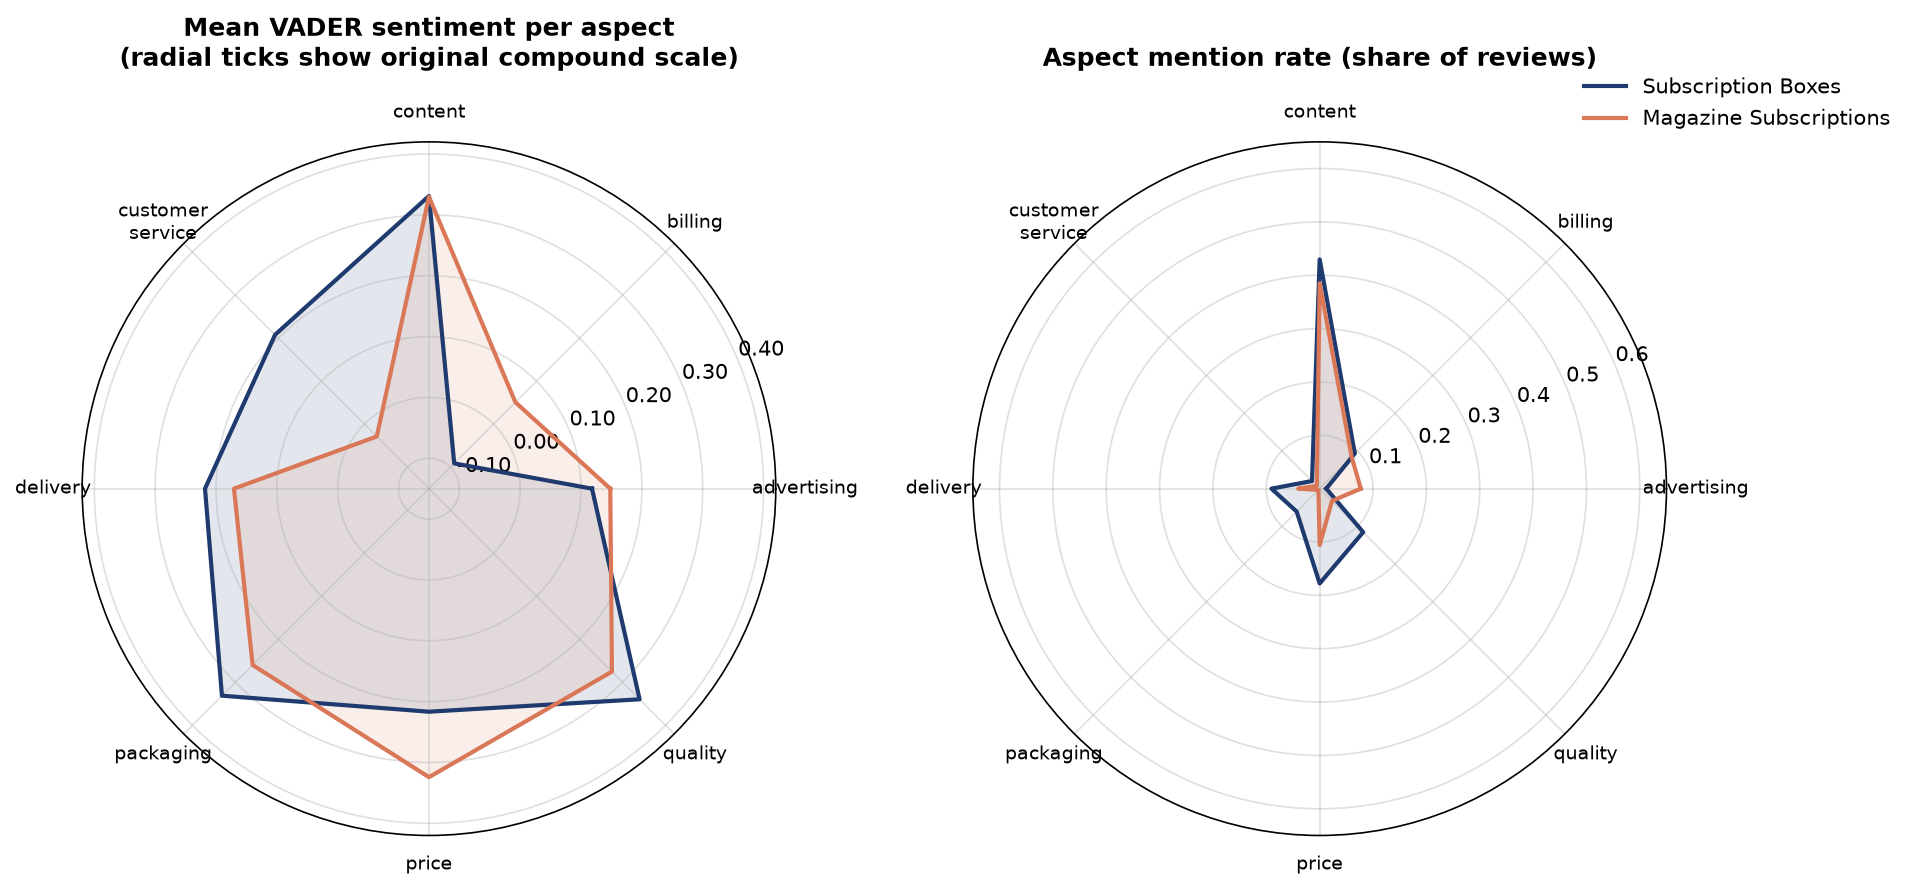
\includegraphics[width=\textwidth]{rq2_aspect_radar.png}
\caption{Aspect profiles as radar charts, with a dynamic, nonclipping radial
range (see Section \ref{sec:method-rq2}). Left: mean VADER sentiment, plotted
via $(\text{compound}+1)/2$ for polar geometry but labelled on the original
$[-1,1]$ scale; billing is the weakest high coverage aspect in both
categories, with low coverage customer service a separate, lower volume
negative signal for magazines. Right: mention rate; content is common in
both categories, while advertising is high coverage only in magazines.}
\label{fig:rq2radar}
\end{figure}

\begin{table}[H]
\centering
\caption{Per aspect mention rate, mean VADER compound and negative share, by
category. \checkmark marks high coverage aspects (mention rate $\geq 5\%$,
Section \ref{sec:method-coverage}); lowest sentiment among high coverage
aspects is identified in the text.}
\label{tab:rq2}
\setlength{\tabcolsep}{4.5pt}
\begin{tabular}{l rrrc rrrc}
\toprule
& \multicolumn{4}{c}{Subscription Boxes} & \multicolumn{4}{c}{Magazine Subscriptions}\\
\cmidrule(lr){2-5}\cmidrule(lr){6-9}
Aspect & Mention\,\% & Mean & Neg\,\% & HC & Mention\,\% & Mean & Neg\,\% & HC \\
\midrule
advertising      & 1.2  & 0.118 & 21.4 &   & 7.7  & 0.148 & 17.8 & \checkmark \\
billing          & 9.3  & -0.091 & 56.9 & \checkmark & 8.5  & 0.051 & 33.4 & \checkmark \\
content          & 43.0 & 0.331 & 12.9 & \checkmark & 38.5 & 0.330 & 10.3 & \checkmark \\
customer service & 2.0  & 0.208 & 27.7 &   & 0.8  & -0.029 & 47.4 &   \\
delivery         & 9.0  & 0.218 & 20.7 & \checkmark & 4.0  & 0.171 & 14.0 &   \\
packaging        & 6.1  & 0.331 & 15.8 & \checkmark & 0.3  & 0.260 & 14.6 &   \\
price            & 17.8 & 0.217 & 25.0 & \checkmark & 10.6 & 0.324 & 15.7 & \checkmark \\
quality          & 11.5 & 0.340 & 14.5 & \checkmark & 3.3  & 0.275 & 14.4 &   \\
\bottomrule
\end{tabular}
\end{table}

\begin{figure}[H]
\centering
\begin{subfigure}{0.49\textwidth}
  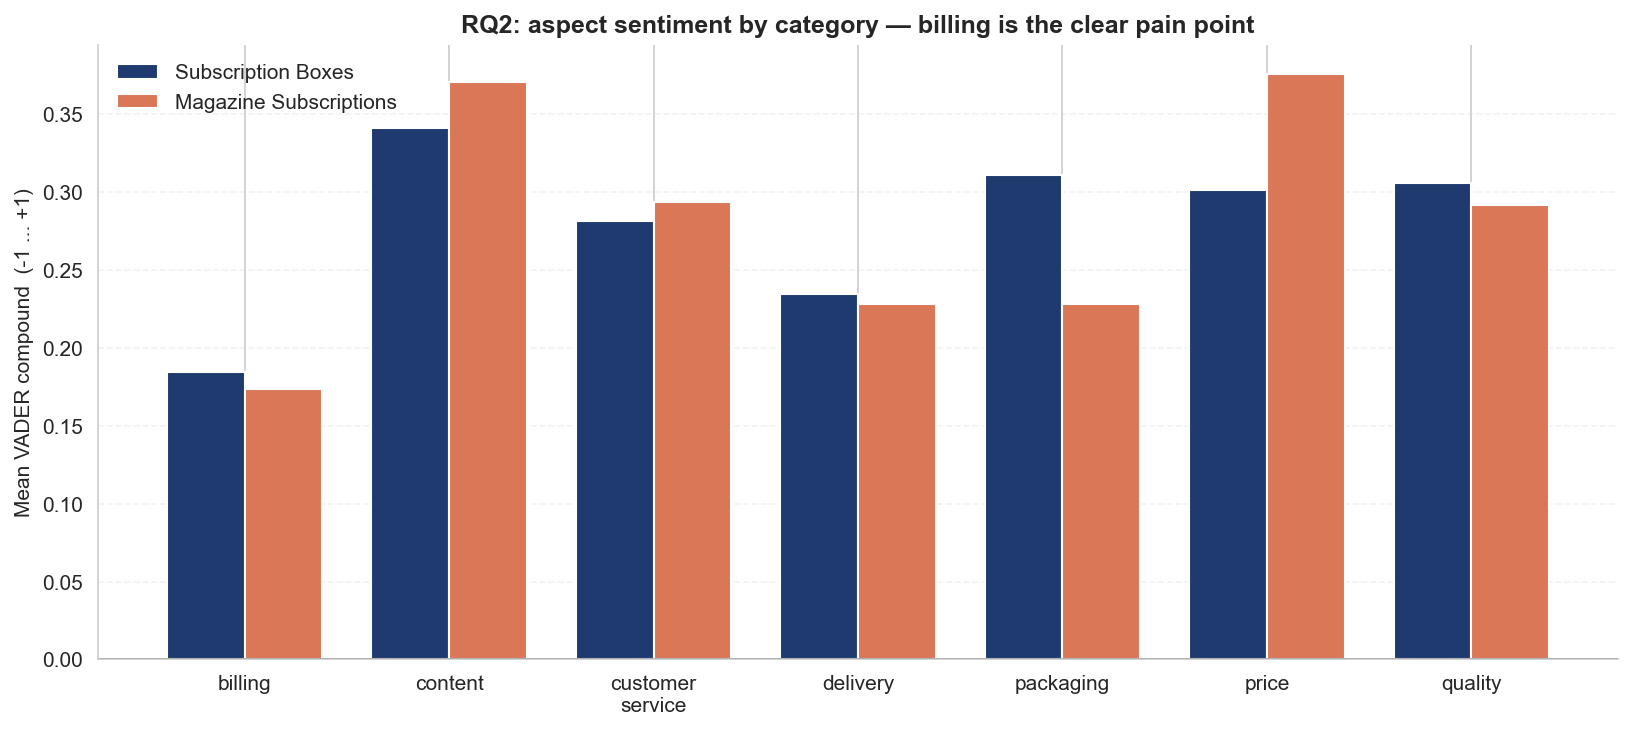
\includegraphics[width=\linewidth]{rq2_aspect_sentiment.png}
  \caption{Mean sentiment per aspect.}
\end{subfigure}\hfill
\begin{subfigure}{0.49\textwidth}
  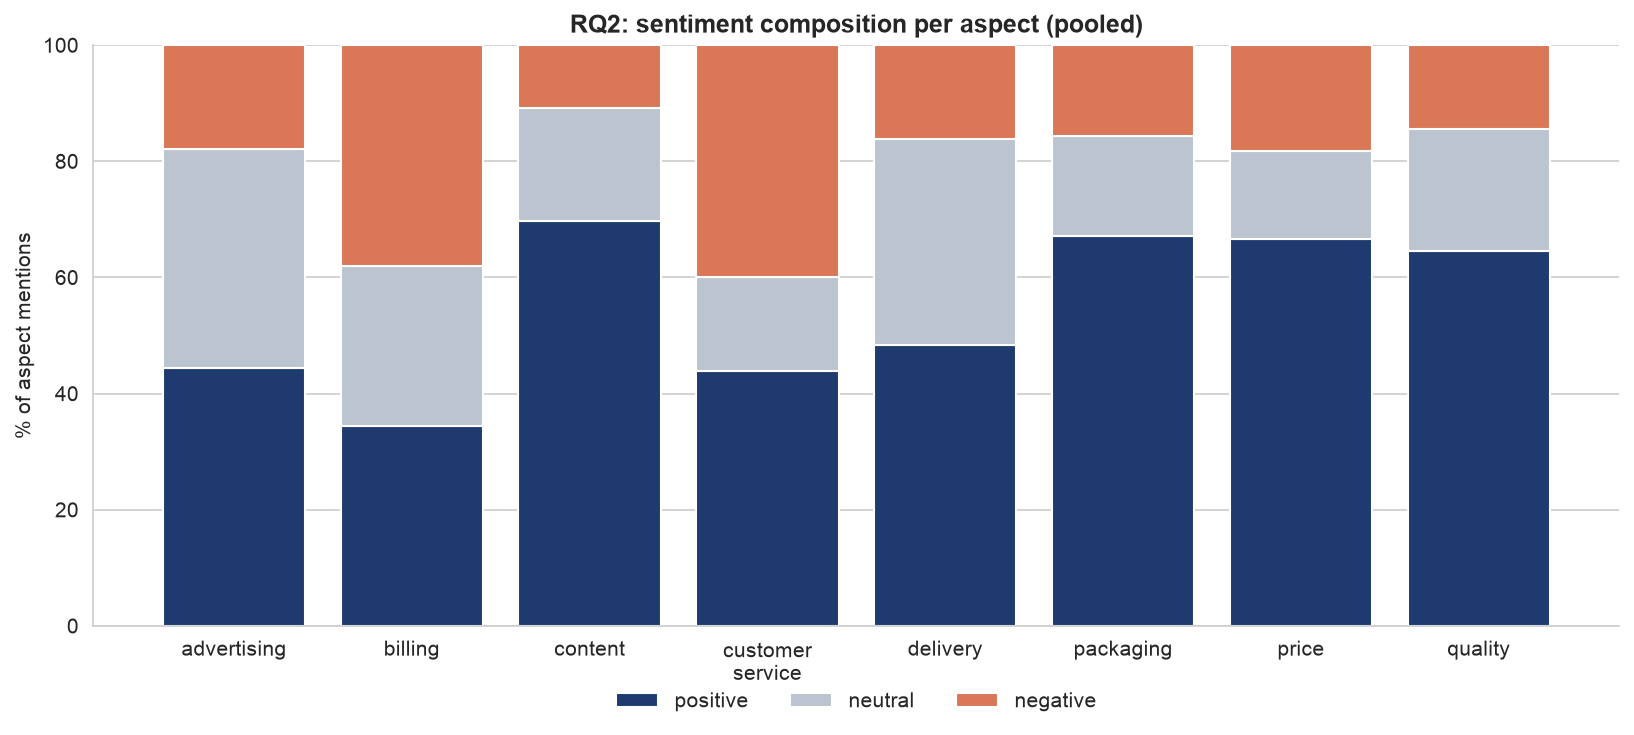
\includegraphics[width=\linewidth]{rq2_sentiment_composition.png}
  \caption{Sentiment composition (pooled).}
\end{subfigure}
\caption{Aspect sentiment as bars and as positive/neutral/negative composition.
Billing is the weakest high coverage aspect in both categories.}
\label{fig:rq2sent}
\end{figure}

\subsection{Noun phrase view}
The most frequent noun phrases (Figure \ref{fig:rq2np}) serve as a useful
stress test rather than a blind validation of the lexicon. Many frequent phrases
are product or category nouns, including the box, this magazine
and the subscription, and are intentionally not mapped to an aspect,
because doing so would recreate the artefact the cleaned lexicon removes. As a
simple keyword versus noun phrase check, $8$ of the top $30$ box phrases and $10$ of
the top $30$ magazine phrases map back to at least one lexicon aspect. Matched
phrases include the toys, the items, the price, ads,
articles and recipes; the unmatched remainder is mostly generic
language, category labels or product names. This makes noun phrases a discovery
check, not a replacement for the curated lexicon.

\begin{figure}[H]
\centering
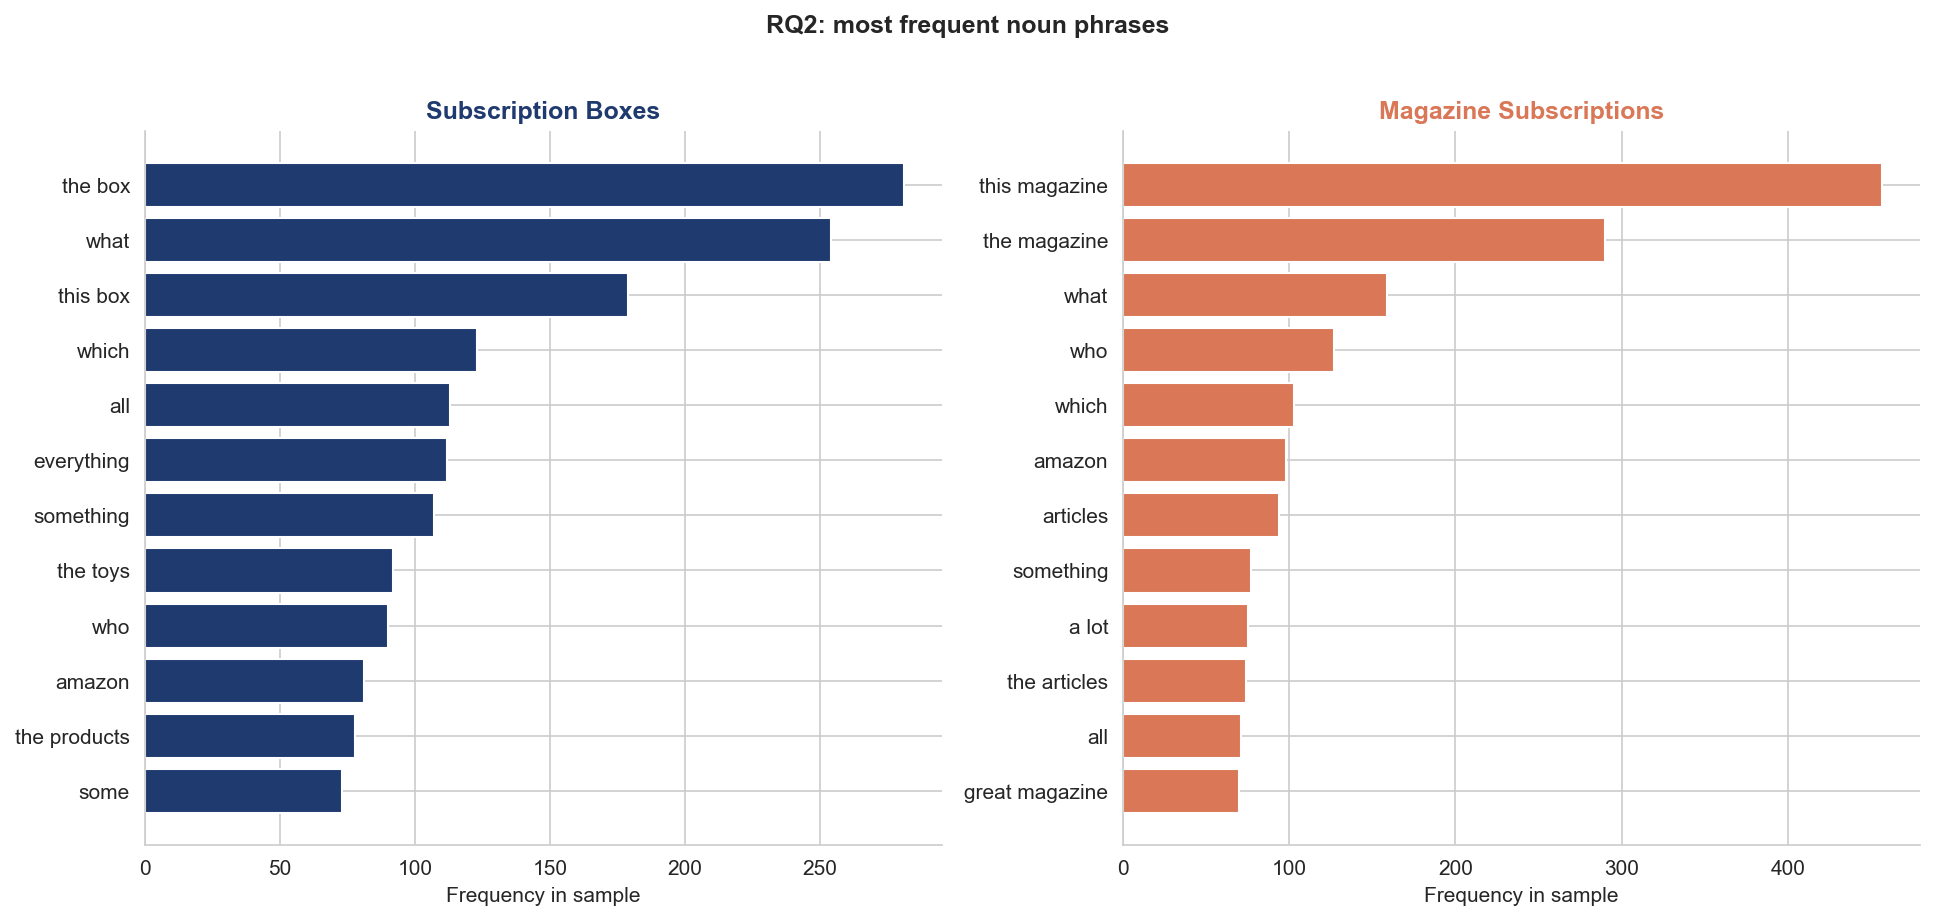
\includegraphics[width=\textwidth]{rq2_noun_phrases.png}
\caption{Most frequent noun phrases per category, a data driven cross check of
the keyword aspect lexicon.}
\label{fig:rq2np}
\end{figure}

\subsection{Robustness: VADER versus the classifier}
\label{sec:rq2-robust}
On a test set sample, VADER and the RQ1 classifier (final selected
configuration, Section \ref{sec:method-split}) agree on $76.8\%$ of
nonneutral aspect mentions ($n=789$; Appendix Table \ref{tab:agree}). VADER labels
$26.1\%$ of sampled aspect mentions as neutral, a category the binary
classifier structurally cannot express. The agreement provides a limited
consistency check between two text based methods, but cannot establish
aspect level validity in the absence of gold annotations. Combined with the
out of distribution concern, this supports using VADER as the primary
sentence level scorer and the classifier as a sanity check only.

\subsection{Illustrative qualitative spot check of the lexicon}
Because no gold aspect labels exist, we inspected a small, deterministic sample
of $80$ aspect assigned sentences (ten per aspect; Appendix \ref{app:val}).
This is not an independent or blinded manual annotation: the
inspection and the resulting judgement were carried out by the author and
encoded directly in the notebook's source code, with no second annotator and
no separately stored annotation file. Under a simple coding rule, a match is
counted as plausible when the sentence explicitly discusses the detected
product or service facet, not merely a category name or a sentiment word,
$77$ of $80$ sampled assignments were judged plausible by the author. This is
reported only as an illustrative qualitative spot check, not as a
validated precision estimate or a gold standard evaluation; the sample is also
too small to support a statistically reliable estimate even if it had been
independently annotated. It does check the highest risk failure modes directly:
box no longer creates packaging hits, subscription no longer
creates billing hits, and sentiment words no longer drive aspect detection. The
remaining limitation is therefore mainly granularity: one sentence can still
mention several aspects and receive one shared VADER score, which the
clause level sensitivity analysis below addresses as a robustness check.

\subsection{Clause level sensitivity analysis}
\label{sec:rq2-clause}
Sentence level attribution remains the primary method, but we directly check
whether it drives the headline findings by rescoring on a conservative
clause split (a semicolon, or one of but, however,
although, though, yet, while, whereas),
attributing each aspect only to the clause containing its keyword,
on a deterministic 8,000 review per category sample. The headline aspect
ranking is essentially unchanged: the rank correlation between
sentence level and clause level aspect sentiment profiles is
$\rho=0.976$ (Subscription Boxes) and $\rho=1.000$ (Magazine Subscriptions,
$n=8$ aspects each). Absolute scores shift slightly more negative at clause
level for almost every aspect (Appendix Table \ref{tab:rq2clause}); billing for
Subscription Boxes moves from $-0.080$ (sentence) to $-0.098$ (clause),
strengthening, not weakening, the billing finding. Among reviews with at
least one detected aspect, $17$ to $22\%$ have at least one aspect whose sentiment
changes when scored from its own clause instead of the whole sentence; reviews
without a detected aspect cannot be affected by this sensitivity check. A
real example shows why this matters: ``This was my first subscription box and
I really enjoy it. I had a little problem with an item that was damaged during
shipping, but the customer service was super nice about it and sent out a
replacement right away.'' At sentence level, content (triggered by
item) inherits the whole second sentence's positive compound ($0.812$,
dominated by ``super nice'', ``replacement right away''); at clause level,
content is correctly scored from its own clause alone ($-0.649$),
while customer\_service keeps the positive clause. The main RQ2
findings are not revised by this analysis, since it does not reverse them;
it mildly reinforces the billing result.

\subsection{Billing lexicon sensitivity check}
\label{sec:rq2-lexicon-check}
Several billing keywords carry negative VADER valence in isolation:
cancel/cancelled score $-0.250$, charged scores $-0.202$,
and charges scores $-0.273$, while most others (refund,
billing, renewal, \ldots) score $0.0$ alone. We therefore recompute billing
sentiment with the matched keyword masked out before VADER scoring and compare
to the unmasked score on the same sentences. Masking shifts mean sentiment
notably toward positive in both categories: Magazine Subscriptions
$0.036\rightarrow0.085$ ($+0.049$); Subscription Boxes
$-0.080\rightarrow+0.044$ ($+0.124$, reversing the sign). This is an
important, honest caveat: a meaningful part of the unmasked billing negative
finding, especially for Subscription Boxes, reflects the lexicon valence of
words like cancel and charged themselves, not solely the
surrounding review context. We do not adopt the masked variant as a new
primary method because masking also strips genuine sentiment bearing context in
many sentences (e.g.\ ``terrible, they keep charging me after I
cancelled'', where terrible and the surrounding clause carry sentiment
that survives masking), but report it as a transparent limitation on how
strongly the unmasked billing finding should be read as purely
context driven.

\subsection{Uncertainty: review level bootstrap}
\label{sec:rq2-uncertainty}
Because several aspect sentence rows can come from the same review, we
resample whole reviews (not rows) for 95\% bootstrap CIs of mean aspect
sentiment per category and of the cross category difference (2,000
replications, fixed seed; Appendix Table \ref{tab:rq2bootstrap}). The underlying code
and CSV name the difference column after the actual category names (Magazine
Subscriptions minus Subscription Boxes), so the direction cannot be misread
from an abstract "a"/"b" convention. The billing
difference (Magazine $-$ Boxes, compound) is $+0.142$, 95\% CI $[0.122, 0.161]$,
which excludes zero, so we describe a stable cross category difference under
this sample. Price is also higher for Magazine than Boxes ($+0.108$, CI
$[0.091, 0.126]$, excludes zero), while quality is higher for Boxes than
Magazine ($-0.064$ Magazine minus Boxes, CI $[-0.089, -0.039]$, excludes
zero). Content's cross category difference CI ($[-0.010, 0.008]$)
includes zero, so we do not claim a stable difference there.

% ============================ 7 DISCUSSION ==================================
\section{Discussion}
\label{sec:discussion}

\paragraph{Performance versus interpretability (Main RQ).}
Logistic Regression is the strongest observed model under the
evaluated setup without sacrificing feature level interpretability. The
balanced binary model reaches macro-F1 $0.888$ on the final test set, ahead of
Gradient Boosting in both the matched sample comparison ($0.876$ vs.\
$0.815$, identical 12,000 row training set, Section \ref{sec:rq1-fair}) and the
full data comparison against Naive Bayes ($0.888$ vs.\ $0.857$, each with its
own validation selected hyperparameters). Because
Logistic Regression wins even when every model family sees identical training
data, this conclusion does not rest on Gradient Boosting having been given
less data, and we do not extrapolate it into a general claim that linear
models are categorically superior to gradient boosting outside this evaluated
setup.

\paragraph{Complementary evidence for billing.}
The strongest negative coefficient of the supervised classifier is the general
negation cue not; among domain specific features, cancel is the
strongest and the fifth largest negative coefficient overall. The
sentence level VADER pipeline also identifies billing as the weakest
high coverage aspect in both categories. These two analyses provide
complementary, triangulating evidence for billing related
dissatisfaction as a recurring subscription product signal, rather than one
independently confirming the other, since both ultimately rely on overlapping
billing related vocabulary. The billing lexicon masking check (Section
\ref{sec:rq2-lexicon-check}) makes this connection explicit and shows its
limit: masking the matched keyword shifts billing sentiment notably toward
positive in both categories (reversing the sign for Subscription Boxes), so
part of the billing negative finding is the lexicon's own valence rather than
purely the surrounding review context.

\paragraph{Label noise candidates and the neutral class.}
Several of the highest confidence errors appear to reflect disagreement between
the rating and the review text, and the ternary results showed that the 3 star
class cannot be reliably separated under this bag of words setup. Both point to
the same limitation: the star rating is a noisy, coarse label, and many of the
hardest reviews are mixed or context poor, exactly where aspect level
analysis can add value over a single document label. The dedicated 3 star
analysis (Section \ref{sec:rq1-3star}) shows this is consistent with a
representational limitation rather than a confidence problem: predicted class
confidence alone does not reliably separate correct from incorrect
predictions here, and bag of words features cannot reliably tell
mildly positive from mildly negative phrasing apart.

\paragraph{Business implications.}
A practitioner can deploy the balanced Logistic Regression as a transparent
polarity monitor, and the lexicon+VADER layer as an aspect dashboard that
flags which facet drives sentiment. Billing is the weakest
high coverage aspect in both categories; complaint language around it is
frequent and scores negative under the lexicon, but the billing lexicon
masking check (Section \ref{sec:rq2-lexicon-check}) shows this negative
polarity is not robust for Subscription Boxes once the triggering
terms are masked out, so for Boxes the aspect's value lies primarily in its
high mention rate and refund/cancel volume rather than in a confidently
negative sentiment score (Magazine Subscriptions is only slightly positive on
billing, so not an unconditional issue there either). For Boxes specifically,
the operational response is still to review renewal, cancellation and refund
flows, monitoring billing negative share and refund/cancel mention rate.
Advertising is a
magazine specific signal worth tracking alongside churn; boxes otherwise need
closer monitoring of content, price and delivery. Difficult 3 star reviews are
better treated as candidates for aspect level review than forced into a single
polarity label. Because both categories are subscription products (Section
\ref{sec:limitations}), these recommendations need fresh validation before
extending to other Amazon categories.

% ============================ 8 LIMITATIONS =================================
\section{Limitations and Future Work}
\label{sec:limitations}

\begin{itemize}[leftmargin=1.4em]
  \item Sentence level attribution is the primary method and cannot,
  by itself, separate two aspects that cooccur in one sentence with mixed
  sentiment (``great content \dots but overpriced''). The clause level
  sensitivity analysis (Section \ref{sec:rq2-clause}) probes this directly,
  but remains a sensitivity check, not a redesigned primary method.
  \item Lexicon and scorer are hand built and English only, and VADER is
  general purpose rather than domain tuned \citep{taboada2011lexicon}; the
  billing lexicon masking check (Section \ref{sec:rq2-lexicon-check}) is a
  partial, not exhaustive, probe of this concern. The content lexicon
  in particular includes broad terms (item, product, issue) so that it
  can match generic mentions of what is being reviewed; for Magazine
  Subscriptions issue is ambiguous between ``magazine issue'' and
  ``problem'', so part of content's high coverage there reflects lexicon
  breadth rather than substantive discussion alone.
  \item No gold aspect labels exist, so RQ2 is validated only against a
  second method and an illustrative, self conducted qualitative
  spot check (not an independent or blinded annotation), not ground truth. A
  small annotated set (SemEval style, \citealp{pontiki2014semeval}) with a
  second, independent annotator would enable proper scoring.
  \item Star ratings as labels are noisy, as the exploratory error
  categorisation suggests (these are possible label noise candidates, not
  confirmed label noise), placing a ceiling on supervised accuracy.
  \item Hyperparameter and feature search used a small, deterministic
  grid (Section \ref{sec:method-split}), not an exhaustive search, to keep
  notebook runtime realistic for a seminar project; a larger search could shift
  the selected configuration.
  \item Cross category scope: both categories studied are subscription
  products, so RQ2's cross category comparison is within a fairly narrow
  product domain and should not be generalised to arbitrary Amazon categories
  without further checks. Subscription Boxes has only 641 distinct items, so
  its aspect frequencies can be influenced by a few popular boxes; the two
  categories also differ in average review length, which is why mention rates
  are also reported per 100 words as a sensitivity check.
  \item Associative, not causal: all RQ1 and RQ2 findings, including
  the billing connection across the two analyses, are descriptive and
  associative.
  \item Neural contrast: a transparent linear model was the goal here; a
  controlled comparison against a Sentence-BERT classifier
  \citep{reimers2019sentencebert} would quantify the interpretability and accuracy
  frontier more precisely.
\end{itemize}

% ============================ 9 CONCLUSION ==================================
\section{Conclusion}
\label{sec:conclusion}

We built a classical NLP pipeline, reproducible given the specified dataset and
environment, that turns 87{,}713 Amazon subscription reviews into structured
opinion data. For document level polarity, across the evaluated models,
imbalance handling had a larger observed effect on minority class performance
than classifier choice: a $69\%$ accurate baseline identifies no negatives, and
only after explicit rebalancing do the models recall the minority class well,
with an interpretable balanced Logistic Regression the strongest
observed model ($0.888$ macro-F1, final test) under the evaluated setup. This is
supported by a matched sample comparison that reduces the concern that the
result is only a training data volume artefact, and reported with bootstrap
confidence intervals rather than as bare point estimates. A direct analysis of true 3 star test reviews shows
the ternary model's persistent difficulty under this setup is consistent with
a representational limitation rather than a confidence problem, since
confidence alone does not reliably separate correct from incorrect
predictions. For aspect based
sentiment, a sentence level lexicon+VADER pipeline (cross checked with a
clause level sensitivity analysis, a billing lexicon masking check, and
review level bootstrap CIs) shows that what customers discuss is mostly
content, while what frustrates them is shared and concentrated in
billing, the weakest high coverage aspect in both categories.
Billing complaint language is frequent and scores negative under the lexicon,
but its polarity is not robust for Subscription Boxes specifically: the
masking check shows the negative skew there largely depends on the
triggering terms (cancel, refund, charged) themselves
rather than on surrounding review context alone. The fact that
the interpretable classifier's strongest domain specific negative word is
cancel, the same billing signal, means the two analyses provide
complementary, triangulating evidence rather than independent confirmation,
and all results here remain associative and descriptive, not causal,
restricted to two subscription product categories rather than Amazon
categories in general.

% ============================ REFERENCES ====================================
\bibliographystyle{plainnat}
\bibliography{references}

% ============================ APPENDIX ======================================
\appendix
\section{Additional material}
\label{app:val}
The repository (\url{https://github.com/ivelinayna/seminar}) contains, under
\texttt{results/tables/}: the full validation slice imbalance handling grid
behind Table \ref{tab:rq1demo}; per class precision/recall/F1; the
hyperparameter search, fair model family, bootstrap CI, 3 star,
clause level and billing lexicon sensitivity, and top noun phrase tables; and the
sentences used for the lexicon spot check (self conducted, not independent or
blinded). It also includes a \texttt{pytest} suite (\texttt{tests/}); all
notebooks reproduce every figure and table from raw data; see
\texttt{README.md} for commands, environment, and seeds.

\begin{table}[H]
\centering
\caption{Strongest Logistic Regression coefficients (binary, balanced, final selected model).}
\label{tab:coef}
\begin{tabular}{lr@{\qquad}lr}
\toprule
Positive term & Weight & Negative term & Weight \\
\midrule
love         & $+15.2$ & not                 & $-11.9$ \\
great        & $+10.5$ & not worth           & $-9.3$ \\
not wait     & $+9.2$  & disappointed        & $-8.8$ \\
enjoy        & $+8.5$  & disappointing       & $-7.4$ \\
good         & $+7.7$  & cancel              & $-7.4$ \\
favorite     & $+7.2$  & not recommend       & $-6.8$ \\
perfect      & $+7.0$  & poor                & $-6.7$ \\
not disappoint & $+6.9$ & horrible          & $-6.2$ \\
\bottomrule
\end{tabular}
\end{table}

\begin{table}[H]
\centering
\caption{Agreement between VADER and the document classifier on nonneutral aspect mentions (test sample).}
\label{tab:agree}
\begin{tabular}{lrr}
\toprule
Aspect & Agreement & $n$ \\
\midrule
advertising      & 0.512 & 43 \\
billing          & 0.737 & 95 \\
content          & 0.791 & 392 \\
customer service & 0.769 & 13 \\
delivery         & 0.867 & 45 \\
packaging        & 0.933 & 15 \\
price            & 0.735 & 132 \\
quality          & 0.815 & 54 \\
\midrule
Overall & 0.768 & 789 \\
\bottomrule
\end{tabular}
\end{table}

\begin{table}[H]
\centering
\caption{Class stratified bootstrap 95\% CIs (2,000 replications), final test set.}
\label{tab:rq1bootstrap}
\begin{tabular}{llrrr}
\toprule
Framing & Metric & Point & CI low & CI high \\
\midrule
Binary  & Accuracy          & 0.902 & 0.897 & 0.906 \\
Binary  & Macro-F1          & 0.888 & 0.883 & 0.893 \\
Binary  & Recall positive   & 0.910 & 0.904 & 0.915 \\
Binary  & Recall negative   & 0.884 & 0.875 & 0.893 \\
\midrule
Ternary & Accuracy          & 0.785 & 0.779 & 0.791 \\
Ternary & Macro-F1          & 0.644 & 0.636 & 0.652 \\
Ternary & Recall positive   & 0.848 & 0.841 & 0.854 \\
Ternary & Recall neutral    & 0.448 & 0.421 & 0.475 \\
Ternary & Recall negative   & 0.731 & 0.719 & 0.743 \\
\bottomrule
\end{tabular}
\end{table}

\begin{table}[H]
\centering
\caption{Rule based exploratory categorisation of the 100 highest confidence binary Logistic Regression errors (final test set).}
\label{tab:err}
\begin{tabular}{lrr}
\toprule
Error category & Count & Share \\
\midrule
Potential rating text disagreement / possible label noise candidate & 47 & 47.0\,\% \\
Very short or context free review                & 25 & 25.0\,\% \\
Mixed sentiment                                  & 14 & 14.0\,\% \\
Domain ambiguity                                 & 8  & 8.0\,\% \\
Probable genuine model error                     & 4  & 4.0\,\% \\
Aspect conflict                                  & 1  & 1.0\,\% \\
Negation                                         & 1  & 1.0\,\% \\
\bottomrule
\end{tabular}
\end{table}

\begin{table}[H]
\centering
\caption{Sentence level vs.\ clause level mean VADER compound, by aspect (8,000 review per category sample).}
\label{tab:rq2clause}
\setlength{\tabcolsep}{3.5pt}
\scriptsize
\begin{tabular}{lrrr@{\qquad}rrr}
\toprule
& \multicolumn{3}{c}{Subscription Boxes} & \multicolumn{3}{c}{Magazine Subscriptions} \\
\cmidrule(lr){2-4}\cmidrule(lr){5-7}
Aspect & Sent. & Clause & Diff & Sent. & Clause & Diff \\
\midrule
advertising      & 0.076 & 0.063 & -0.013 & 0.171 & 0.139 & -0.032 \\
billing          & -0.080 & -0.098 & -0.018 & 0.036 & 0.020 & -0.016 \\
content          & 0.332 & 0.321 & -0.011 & 0.322 & 0.307 & -0.015 \\
customer service & 0.176 & 0.181 & 0.005 & 0.013 & -0.001 & -0.014 \\
delivery         & 0.233 & 0.213 & -0.021 & 0.179 & 0.146 & -0.033 \\
packaging        & 0.330 & 0.324 & -0.006 & 0.252 & 0.241 & -0.010 \\
price            & 0.221 & 0.200 & -0.021 & 0.316 & 0.303 & -0.013 \\
quality          & 0.348 & 0.341 & -0.007 & 0.307 & 0.288 & -0.019 \\
\bottomrule
\end{tabular}
\end{table}

\begin{table}[H]
\centering
\caption{Review level bootstrap 95\% CIs for mean aspect sentiment (2,000 replications). Diff column is Magazine Subscriptions minus Subscription Boxes.}
\label{tab:rq2bootstrap}
\setlength{\tabcolsep}{3.5pt}
\scriptsize
\begin{tabular}{lrrr}
\toprule
Aspect & Mean (Boxes) [CI] & Mean (Magazine) [CI] & Diff (Mag.$-$Boxes) [CI] \\
\midrule
advertising & 0.118 [0.059, 0.173] & 0.148 [0.139, 0.157] & 0.030 [-0.026, 0.088] \\
billing & -0.091 [-0.109, -0.074] & 0.051 [0.042, 0.060] & 0.142 [0.122, 0.161] \\
content & 0.331 [0.322, 0.340] & 0.330 [0.326, 0.334] & -0.001 [-0.010, 0.008] \\
customer service & 0.208 [0.152, 0.262] & -0.029 [-0.065, 0.008] & -0.236 [-0.302, -0.172] \\
delivery & 0.218 [0.196, 0.239] & 0.171 [0.158, 0.184] & -0.048 [-0.073, -0.021] \\
packaging & 0.331 [0.306, 0.357] & 0.260 [0.213, 0.309] & -0.071 [-0.128, -0.017] \\
price & 0.217 [0.201, 0.231] & 0.324 [0.315, 0.334] & 0.108 [0.091, 0.126] \\
quality & 0.340 [0.321, 0.359] & 0.275 [0.258, 0.292] & -0.064 [-0.089, -0.039] \\
\bottomrule
\end{tabular}
\end{table}

\bigskip
\begin{center}Declaration of Originality\end{center}
\noindent
I declare that I have authored this paper independently, that I have not used
other than the declared sources / resources, and that I have explicitly marked
all material which has been quoted either literally or by content from the used
sources.
\vspace{1.5cm}

\noindent
\theplace, \thedate \hfill
\begin{tabular}{c}
{\Large\calligra Yaneva}\\[-0.6ex]
\rule{6cm}{0.4pt}\\[-0.1ex]
\theauthor
\end{tabular}

\end{document}
